% !TEX root = saveliev_physics_general_course_1.tex
%!TEX TS-program = pdflatex
%!TEX encoding = UTF-8 Unicode


\chapter{CÁC ĐỊNH LUẬT BẢO TOÀN}\label{chap:3}

\section{Các đại lượng được bảo toàn}\label{sec:3_1}

Các vật tạo thành hệ cơ học có thể tương tác với nhau cũng như các vật không phụ thuộc hệ này. Ứng với điều này có thể chia các lực tác dụng lên các vật của hệ thành \textbf{nội lực} và \textbf{ngoại lực} . Ta sẽ gọi các lực mà các vật còn lại của hệ tác động lên vật đã cho là các nội lực, và các lực được gây bởi tác động của các vật không thuộc hệ là các ngoại lực.

Trong trường hợp nếu không có các ngoại lực thì hệ được gọi là \textbf{hệ kín}.

Đối với các hệ kín tồn tại các hàm của các tọa độ và của vận tốc của các hạt tạo thành hệ\footnote{Ta hãy nhớ rằng, để ngắn gọn ta gọi chất điểm là hat.} giữ nguyên giá trị không đổi khi chuyển động. Các hàm này được gọi là các \textbf{tích phân chuyển động}.

Đối với một hệ gồm $N$ hạt mà giữa chúng không có các liên kết rắn thì có thể thành lập được $6N-1$ tích phân chuyển động. Tuy nhiên trong chúng người ta chỉ quan tâm đến các tích phân chuyển động có tính chất cộng tính. Tính chất này có nội dung là giá trị của tích phân chuyển động đối với hệ gồm các hạt mà có thể bỏ qua tương tác của chúng, bằng tổng các giá trị của tích phân chuyển động đối với từng hạt tách biệt. Có ba tích phân chuyển động cộng tính. Một trong chúng được gọi là \textbf{năng lượng}, cái thứ hai là \textbf{xung lượng}, và cái thứ ba là \textbf{momen xung lượng}.

Như vậy đối với các hệ kín có ba đại lượng vật lý không biến đổi (được bảo toàn): năng lượng, xung lượng và momen xung lượng. Ứng với điều này có \textbf{ba định luật bảo toàn}---định luật bảo toàn năng lượng, định luật bảo toàn xung lượng và định luật bảo toàn momen xung lượng. Các định luật này liên hệ chặt chẽ với các tính chất cơ bản của không gian và thời gian.

\textbf{Sự đồng tính của thời gian} là cơ sở của sự bảo toàn năng lượng, nghĩa là tính tương đương của tất cả các thời điểm. Cần hiểu tính tương đương theo nghĩa là sự thay thế thời điểm $t_1$ bằng thời điểm $t_2$ mà không làm biến đổi giá trị của các tọa độ và vận tốc của các hạt thì sẽ không làm biến đổi các tính chất cơ học của hệ. Điều này có nghĩa là sau sự thay thế nói trên các tọa độ và vận tốc của các hạt tại thời điểm $t_2+t$ bất kỳ cũng sẽ có cùng các giá trị mà chúng đã có tại thời điểm $t_1+t$ trước khi thay thế.

\textbf{Sự đồng tính của không gian} là cơ sở của sự bảo toàn xung lượng, nghĩa là sự đồng nhất của các tính chất của không gian tại mọi điểm. Cần phải hiểu sự đồng nhất theo nghĩa là khi dịch chuyển song song một hệ kín từ chỗ này trong không gian sang chỗ kia mà không thay đổi vị trí tương hỗ và các vận tốc của hạt thì sẽ không làm biến đổi các tính chất cơ học của hệ (giả sử rằng ở chỗ mới tính kín của hệ không bị phá hủy). 

Sau cùng, \textbf{tính đẳng hướng của không gian} là cơ sở của sự bảo toàn momen xung lượng, nghĩa là sự đồng nhất của các tính chất của không gian theo mọi hướng. Cần phải hiểu sự đồng nhất theo nghĩa là sự quay một hệ kín hoàn toàn không ảnh hưởng tới các tính chất cơ học của hệ.

Các định luật bảo toàn là một vũ khí rất có hiệu lực của việc nghiên cứu. Thông thường lời giải chính xác của phương trình chuyển động là rất phức tạp. Trong những trường hợp này nhờ các định luật bảo toàn có thể thu được một loạt dữ kiện quan trọng về sự diễn biến của các hiện tượng cơ học mà không phải giải các phương trình chuyển động. Các định luật bảo toàn không phụ thuộc vào đặc tính của các lực tác dụng. Do đó, nhờ chúng có thể thu được một loạt thông tin quan trọng về trạng thái của các hệ cơ học ngay cả trong các trường hợp khi các lực đều chưa biết.

Trong các tiết sau ta sẽ thu được các định luật bảo toàn xuất phát từ các phương trình Newton. Tuy nhiên cần chú ý rằng các định luật bảo toàn có tính tổng quát lớn hơn các định luật Newton rất nhiều. Các định luật bảo toàn thực sự vẫn còn đúng ngay cả khi các định luật Newton (cụ thể là định luật thứ ba) bị vi phạm. Ta hãy nhấn mạnh rằng các định luật bảo toàn năng lương, xung lượng và momen xung lượng là các đinh luật chính xác cũng đúng là một cách nghiêm ngặt cả trong lĩnh vực tương đối tính.

\section{Động năng}\label{sec:3_2}

Ta bắt đầu tìm các tích phân chuyển động cộng tính. Để bắt đầu ta xét hệ đơn giảm gồm một hạt (một chất điểm).

Ta viết phương trình chuyển động của hạt:
\begin{equation}\label{eq:3_1}
m\dot{\vec{v}} = \vec{F}.
\end{equation}

\noindent
Ở đây $\vec{F}$ là lực tổng hợp tác dụng lên hạt. Nhân phương trình~\eqn{3_1} với độ dịch chuyển của hạt $\mathrm{d}\vec{s}=\vec{v}\,\mathrm{d}t$, ta có:
\begin{equation}\label{eq:3_2}
m\vec{v}\dot{\vec{v}}\,\mathrm{d}t = \vec{F}\,\mathrm{d}\vec{s}.
\end{equation}

\noindent
Tích $\dot{\vec{v}}\,\mathrm{d}t$ là số gia $\mathrm{d}\vec{v}$ của vận tốc hạt trong thời gian $\mathrm{d}t$. Một cách tương ứng
\begin{equation}\label{eq:3_3}
m\vec{v}\dot{\vec{v}}\,\mathrm{d}t = m\vec{v}\,\mathrm{d}\vec{v} = m\,\mathrm{d}\!\left(\frac{v^2}{2}\right) = \mathrm{d}\!\left(\frac{mv^2}{2}\right)
\end{equation}

\noindent
%[see \eqn{2_50}].
Nếu thay thế vào \eqn{3_2}, ta đi tới hệ thức
\begin{equation}\label{eq:3_4}
\mathrm{d}\!\left(\frac{mv^2}{2}\right) = \vec{F}\,\mathrm{d}\vec{s}.
\end{equation}

\noindent
Nếu hệ kín, $\vec{F}=0$, thì $\mathrm{d}(mv^2/2)=0$, còn chính đại lượng
\begin{equation}\label{eq:3_5}
E_{\text{k}} = \frac{mv^2}{2}
\end{equation}

\noindent
vẫn không đổi. Đại lượng này được gọi là \textbf{động năng} của hạt. Trong trường hợp một hạt cô lập, động năng là một tích phân chuyển động\footnote{Trong trường hợp một hạt cô lập thì bất kỳ mức nào của vận tốc vẫn không đổi. Tuy nhiên trong trường hợp hệ gồm số hạt tương tác với nhau thì chính các đại lượng có dạng~\eqref{eq:3_5} sẽ tham gia vào các tích phân chuyển động cộng tính như các số hạng. }.

Nhân tử số và mẫu số của biểu thức~\eqref{eq:3_5} với $m$ và để ý rắng tích số $mv$ bằng xung lượng $p$ của vật, có thể cho biểu thức đối với động năng dạng:
\begin{equation}\label{eq:3_6}
E_{\text{k}} = \frac{p^2}{2m}.
\end{equation}

\noindent
Nếu lực $\vec{F}$ tác dụng lên hạt thì động năng sẽ thay đổi. Trong trường hợp này theo~\eqref{eq:3_4} số gia của động năng của hạt trong thời gian $\mathrm{d}\vec{t}$ bằng tích vô hướng $\vec{F}\,\mathrm{d}\vec{s}$ ($\mathrm{d}\vec{s}$ là độ dời của hạt trong thời gian $\mathrm{d}t$). Đại lượng 
\begin{equation}\label{eq:3_7}
\mathrm{d}A = \vec{F}\,\mathrm{d}\vec{s}
\end{equation}

\noindent
được coi là \textbf{công} do lực $\vec{F}$ thực hiện trên quãng đường $\mathrm{d}s$ ($\mathrm{d}s$ là module độ rời $\mathrm{d}\vec{s}$). Có thể biểu diễn tích vô hướng \eqref{eq:3_7} dưới dạng tích của các hình chiếu của lực trên hướng chuyển dời $F_{\text{s}}$ và của yếu tố đường đi $\mathrm{d}s$. Do đó có thể viết là 
\begin{equation}\label{eq:3_8}
\mathrm{d}A = F_{\text{s}}\,\mathrm{d}s.
\end{equation}

\noindent
Từ điều đã nói rõ ràng rằng công đặc trưng cho sự biến đổi năng lượng gây ra bởi tác dụng của lực lên hạt chuyển động.

Ta hãy lấy tích phân hệ thức~\eqref{eq:3_4} dọc theo quỹ một quỹ đạo nào đó từ điểm $1$ đến điểm $2$:
\begin{equation*}
\int_{1}^{2} \mathrm{d}\!\left(\frac{mv^2}{2}\right) = \int_{1}^{2} \vec{F}\,\mathrm{d}\vec{s}.
\end{equation*}

\noindent
Vế trái là hiệu các giá trị của động năng tại các điểm $2$ và $1$, tức là số gia\footnote{Có thể đặc trưng sự biển đổi của đại lượng $a$ nào đó hoặc bằng số gia hoặc bằng độ giảm của nó. Người ta gọi hiệu của giá trị cuối ($a_2$) và giá trị ban đầu ($a_1$) của đại lượng $a$ là số gia của đại lượng này và ta sẽ ký hiệu nó bằng $\Delta a$: 

$\text{số gia}=\Delta a=a_2-a_1$. 

Người ta gọi độ giảm của đại lượng $a$ là hiệu của giá trị ban đầu ($a_1$) và giá trị cuối ($a_2$): 

$\text{độ giảm}=a_1-a_2=-\Delta a$. 

Độ giảm của một đại lượng bằng số gia của nó lấy dấu ngược lại. Số gia và độ giảm là các đại lượng đại số.} của động năng trên quãng đường $1$-$2$. Để ý đến điều đó, ta có:
\begin{equation}\label{eq:3_9}
E_{\text{k},2} - E_{\text{k},1} = \frac{mv^2_2}{2} - \frac{mv^2_1}{2} = \int_{1}^{2} \vec{F}\,\mathrm{d}\vec{s}.
\end{equation}

Đại lượng 
\begin{equation}\label{eq:3_10}
A = \int_{1}^{2} \vec{F}\,\mathrm{d}\vec{s} = \int_{1}^{2} F_{\text{s}}\,\mathrm{d}s
\end{equation}

\noindent
là công của lực $\vec{F}$ trên quãng đường $1$-$2$. Đôi khi ta ký hiệu công này bằng ký hiệu $A_{12}$ thay cho $A$.

Vậy, \textit{công của tất cả các lực tổng hợp tác dụng lên hạt chuyển thành độ tăng động năng của hạt}:
\begin{equation}\label{eq:3_11}
A_{12} = E_{\text{k},2} - E_{\text{k},1}.
\end{equation}

\noindent
Từ \eqn{3_11} suy ra rằng năng lượng có cùng thứ nguyên như công. Ứng với điều này, năng lượng được đo bằng cùng các đơn vị giống như công (xem mục sau).


\section{Công}\label{sec:3_3}

Ta hãy khảo sát đại lượng được gọi là công một cách tỉ mỉ hơn. Có thể biểu diễn biểu thức~\eqref{eq:3_7} dưới dạng
\begin{equation}\label{eq:3_12}
\mathrm{d}A = \vec{F}\,\mathrm{d}\vec{s} = F\cos\alpha\,\deriv{s}
\end{equation}

\noindent
trong đó $\alpha$ là góc giữa hướng của lực và hướng dịch chuyển của điểm đặt lực.

Nếu lực và hướng dịch chuyển tạo thành một góc nhọn  ($\cos\alpha>0$) thì công là dương. Nếu góc $\alpha$ là góc tù ($\cos\alpha<0$) thì công là âm. Với $\alpha=\pi/2$ công bằng không. Điều sau cùng chứng tỏ đặc biệt rõ ràng rằng khái niệm công trong cơ học khác hẳn với khái niệm hàng ngày về công. Trong cách hiểu thông thường, mọi sự nỗ lực, cụ thể là sự căng cơ bắp luôn luôn kèm theo sự thực hiện công. Chẳng hạn, để giữ một vật nặng đứng yên, hơn nữa để dịch chuyển vật này theo quãng đường nằm ngang, người mang sẽ tiêu tốn nhiều sức lực, nghĩa là ``thực hiện công''. Tuy nhiên công như một đại lượng cơ học, trong các trường hợp này là bằng không.

\begin{figure}[!htb]
	\begin{center}
		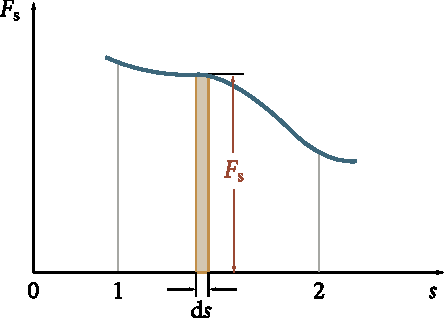
\includegraphics[scale=1]{figures/ch_03/fig_3_1.pdf}
		\caption[]{}
		\label{fig:3_1}
	\end{center}
\end{figure}

Trên hình~\ref{fig:3_1}, trình bày đồ thị hình chiếu  của lực lên hướng dịch chuyển $F_{\text{s}}$ như một hàm của vị trí của hạt trên quỹ đạo (có thể gọi trục hoành là trục $s$, độ dài của đoạn trục này giữa hai điểm $1$ và $2$ bằng độ dài toàn phần của quãng đường). Từ hình vẽ rõ ràng là công nguyên tố $\deriv{A}=F_{\text{s}}\,\deriv{s}$ về trị số bằng diện tích của dải gạch gạch, còn công $A$ trên quãng đường $1$-$2$ về trị số bằng diện tích của hình được được giới hạn bởi đường cong $F_{\text{s}}$, các đường thẳng đứng $1$ và $2$ và trục $s$ (so với \fig{1_26}).

Ta hãy áp dụng kết quả này để tìm công thực hiển trong sự biến dạng của lò xo tuần theo định luật Hooke   (xem \fig{2_5} và công thức \eqref{eq:2_26}). Ta bắt đầu từ sự giãn của lò xo. Ta sẽ thực hiện sự giãn rất chậm để lực $\vec{F}_{\text{ext}}$ mà ta tác dụng lên lò xo có thể luôn luôn được coi bằng lực đàn hồi $\vec{F}_{\text{el}}$ về độ lớn. Khi đó, $\vec{F}_{x,\text{ext}}=-\vec{F}_{x,\text{el}}=kx$, trong đó  $x$ là độ dãn của lò xo (\fig{3_2}). Từ hình vẽ rõ ràng là công cần thực hiện để gây ra độ dãn $x$ của lò xo bằng
\begin{equation}\label{eq:3_13}
A = \frac{kx^2}{2}.
\end{equation}

\noindent
Khi nén lò xo một lượng $x$ thì về độ lớn và về dấu công được thực hiện cũng giống như khi dãn một lượng $x$. Hình chiếu của lực $\vec{F}_{\text{ext}}$ trong trường hợp này là âm ($\vec{F}_{\text{ext}}$ hướng về phía bên trái, $x$ tăng lên về bên phải, xem \fig{3_2}), tất cả $\deriv{x}$ cũng đều âm. Do đó, tích $\vec{F}_{x,\text{ext}}\,\deriv{x}$ là dương.

\begin{figure}[!htb]
	\begin{center}
		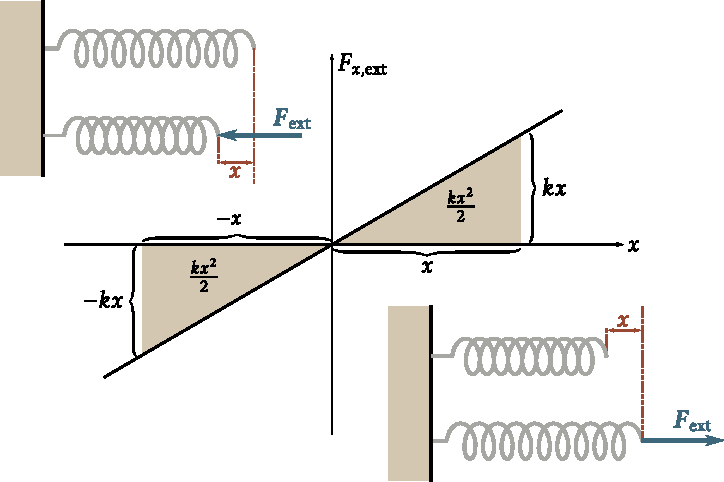
\includegraphics[scale=0.95]{figures/ch_03/fig_3_2.pdf}
		\caption[]{}
		\label{fig:3_2}
	\end{center}
\end{figure}

Một cách tương tự có thể tìm biểu thức đối với công thực hiện khi dãn hoặc nén đàn hồi một thanh. Theo công thức \eqref{eq:2_31}, công này bằng
\begin{equation}\label{eq:3_14}
A = \frac{1}{2}\frac{ES}{l_0}(\Delta l)^2 = \frac{1}{2}ESl_0\left(\frac{\Delta l}{l_0}\right)^2 = \frac{1}{2}EV\varepsilon^2
\end{equation}

\noindent
trong đó $V=Sl_0$ là thể tích của thanh, còn $\varepsilon=\Delta l/l_0$ là độ dãn tỷ đối (xem \eqnref{eq:2_27}).

Giả sử một số lực mà    lực tổng hợp của chúng bằng  $\vec{F}=\sum_{i}\vec{F}_i$ tác dụng đồng thời lên vật. Từ tính phân phối của tích vô hướng của các vector  (xem \eqref{eq:1_20}) suy ra rằng công $\deriv{A}$ thực hiện bởi lực tổng hợp trên quãng đường $\deriv{s}$ có thể được biểu diễn dưới dạng
\begin{equation}\label{eq:3_15}
\deriv{A} = \left(\sum_{i}\vec{F}_i\right)\deriv{s} = \sum_{i}\vec{F}_i\,\deriv{\vec{s}} = \sum_{i}\deriv{A}_i.
\end{equation}

\noindent
Điều này có nghĩa là công của lực tổng hợp của một số lực bằng tổng đại số các công được thực hiện bởi từng lực tách biệt.

Độ dời nguyên tố $\deriv{\vec{s}}$ có thể được biểu diễn như $\vec{v}\deriv{t}$. Do đó có thể cho biểu thức đối với công nguyên tố dạng
\begin{equation}\label{eq:3_16}
\deriv{A} = \vec{F}\vec{v}\,\deriv{t}.
\end{equation}

\noindent
Khi đó thực hiện trong khoảng thời gian $t_1$ đến $t_2$ có thể tính theo công thức
\begin{equation}\label{eq:3_17}
A = \int_{t_1}^{t_2}\vec{F}\,\deriv{t}.
\end{equation}

Ứng với \eqref{eq:1_21} $\vec{F}\,\deriv{\vec{s}}=F\,\deriv{s_F}$, trong đó $\deriv{s_F}$, là hình chiếu của độ dời nguyên tố $\deriv{\vec{s}s}$ lên hướng của lực $\vec{F}$. Do đó có thể viết công thức đối với công như sau:
\begin{equation}\label{eq:3_18}
\deriv{A} = F\,\deriv{s_F}.
\end{equation}

\begin{figure}[!htb]
	\begin{center}
		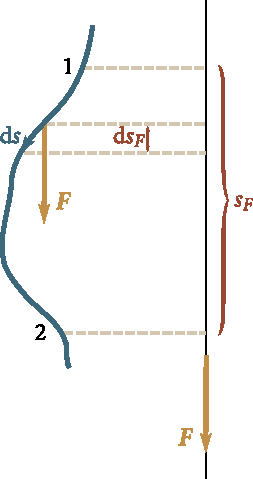
\includegraphics[scale=0.95]{figures/ch_03/fig_3_3.pdf}
		\caption[]{}
		\label{fig:3_3}
	\end{center}
\end{figure}

Nếu lực có độ lớn và hướng không đổi (\fig{3_3}), thì có thể đưa vector $\vec{F}$ trong biểu thức đối với công ra ngoài dấu tích phân, kết quả ta có công thức
\begin{equation}\label{eq:3_19}
A = \vec{F}\int_{1}^{2}\deriv{\vec{v}} = \vecdot{F}{s} = F s_F
\end{equation}

\noindent
trong đó $\vec{s}$ là vector độ dời từ điểm $1$ đến điểm $2$, còn $s_F$ là hình chiếu của nó lên hướng của lực.
Công được thực hiện trong một đơn vị thời gian được gọi là công suất. Nếu công $\deriv{A}$ được thực hiện trong khoảng thời gian $\deriv{t}$ thì công suất bằng
\begin{equation}\label{eq:3_20}
P = \diff{A}{t}.
\end{equation}

\noindent
Nếu lấy $\deriv{A}$ ở dạng \eqref{eq:3_16}, ta được biểu thức đối với công suất 
\begin{equation}\label{eq:3_21}
P = \vecdot{F}{v}
\end{equation}

\noindent
theo biểu thức này công suất bằng tích vô hướng của vector lực với vector vận tốc chuyển động của điểm đặt lực. 

\textbf{Các đơn vị công và công suất.} Để làm đơn vị công người ta dùng công được thực hiện bởi lực bằng một đơn vị và tác dụng theo hướng dịch chuyển bởi lực bằng một đơn vị và tác dụng theo hướng dịch chuyển trên một quãng đường bằng một đơn vị. Một cách tương ứng:
\begin{enumerate}[(1)]
	\item trong hệ SI đơn vị công là jun (\si{\joule}); nó bằng công thực hiện bởi một lực \SI{1}{\newton} trên đoạn đường \SI{1}{\metre};
	\item trong hệ CGS là  \si{\erg}, bằng công thực hiện bởi một lực \SI{1}{\dyne} trên đoạn đường \SI{1}{\centi\metre};
	\item trong hệ MkGS là kilogam lực-mét(\si{\kgf\metre}), bằng công thực hiện bởi một lực  \SI{1}{\kgf} trên đoạn đường \SI{1}{\metre}.
\end{enumerate}

Giữa các đơn vị công có hệ thức
\begin{align*}
&\SI{1}{\joule} = \SI{1}{\newton}\times\SI{1}{\metre} = \SI{e5}{\dyne}\times\SI{e2}{\centi\metre} = \SI{e7}{\erg}\\
&\SI{1}{\kgf\metre} = \SI{1}{\kgf}\times\SI{1}{\metre} = \SI{9.81}{\newton}\times\SI{1}{\metre} = \SI{9.81}{\joule}.
\end{align*}

Người ta thừa nhận công suất do công bằng một đơn vị thực hiện trong một đơn vị thời gian làm đơn vị công suất. Trong hệ SI đơn vị công suất là oát (\si{\watt}), bằng jun trên giây (\si{\joule\per\second}). Đơn vị công suất trong hệ CGS (\si{\erg\per\second}) không có tên gọi riêng. Sự tương quan giữa oát và ec/s: \si{\erg\per\second} là $\SI{1}{\watt}=\SI{e7}{\erg\per\second}$.

Trong hệ MkGS người ta dùng đơn vị công suất là mã lực (\si{\hp}), bằng \SI{75}{\kgf\metre\per\second}, $\SI{1}{\hp}=\SI{736}{\watt}$ (không được nhầm lẫn giữa đơn vị của Anh và Mỹ: 1 mã lực bằng \num{550}~ft-lb \si{\per\second} hoặc \SI{746}{\watt}).

Ngoài các đơn vị đo đã nêu, người ta còn dùng các đơn vị bội và ước. Các tên gọi và ký hiệu của chúng được tạo thành từ tên gọi và ký hiệu của đơn vị cơ bản và các tiếp đầu ngữ đã nêu trong Bảng~\ref{table:3_1}. Trong bảng cũng chỉ rõ các thừa số mà nhờ chúng các đơn vị bội và ước tương ứng được tạo thành từ các đơn vị cơ bản.

\begin{table}[htb!]
	\renewcommand{\arraystretch}{1.2}
	\caption{Các tên gọi và ký hiệu của các tiếp đầu ngữ dùng để tạo thành các đơn vị bội và ước }
	\vspace{-0.6cm}
	\label{table:3_1}
	\begin{center}\resizebox{0.95\linewidth}{!}{
			\begin{tabular}{lcclcc}
				\toprule[1pt]
				\textbf{Tên gọi} & \textbf{Ký hiệu} & \textbf{Thừa số} &
    \textbf{Tên gọi} & \textbf{Ký hiệu} & \textbf{Thừa số}\\
				\midrule[0.5pt]\midrule[0.5pt]
				Tera & T & \num{e12} & Centi & \si{\centi \ } & \num{e-2}\\
				Giga & G & \num{e9} & Milli & \si{\milli \ } & \num{e-3}\\
				Mega & M & \num{e6} & Micro & \si{\micro \ } & \num{e-6}\\
				Kilo & k & \num{e3} & Nano & \si{\nano \ } & \num{e-9}\\
				Hecto & h & \num{e2} & Pico & \si{\pico \ } & \num{e-12}\\
				Deca & da & \num{e1} & Femto & \si{\femto \ } & \num{e-15}\\
				Deci & d & \num{e-1}  & Atto & \si{\atto \ } & \num{e-18}\\
				\bottomrule[1pt]
			\end{tabular}
	}\end{center}
\end{table}

Chẳng hạn, đơn vị công mang tên là megajoule tương đương với  \num{e6} joules ($\SI{1}{\mega\joule}=\SI{e6}{\joule}$), còn đơn vị công suất mang tên là microwatt tương đương với \num{e-6} watt ($\SI{1}{\micro\watt}=\SI{e-6}{\watt}$). Một cách tương tự:  \SI{e-6}{\metre} ($\SI{1}{\micro\metre}=\SI{e-6}{\metre}$),  $\SI{1}{\pico\newton}=\SI{e-12}{\newton}$.

\section{Các lực bảo toàn}\label{sec: 3_3}
Nếu tại mỗi điểm của không gian hạt chịu tác động của các vật khác, thì người ta nói rằng hạt này nằm trong trường lực. Chẳng hạn, hạt ở gần mặt đất nằm trong trọng trường, nghĩa là lực $\vec{P}=m\vec{g}$ tác dụng lên nó tại mỗi điểm của không gian

\begin{figure}[!htb]
	\begin{center}
		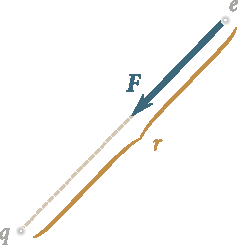
\includegraphics[scale=1]{figures/ch_03/fig_3_4.pdf}
		\caption[]{}
		\label{fig:3_4}
	\end{center}
\end{figure}

Để làm ví dụ thứ hai ta hãy nghiên cứu hạt tích điện $e$ nằm trong điện trường gây bởi tích điểm $q$ đứng yên (\fig{3_4}). Trường này được đặc trưng bằng phương của lực, tác dụng lên hạt tại một diểm bất kỳ của không gian, đi qua tâm đừng yên (điện tích $q$), còn độ lớn của lực chỉ phụ thuộc vào khoảng cách tới tâm này: $F=F(r)$ (xem công thức~\eqref{eq:2_23}). Trường lực có các tính chất như vậy được gọi là \textbf{trường lực xuyên tâm}.

Nếu tại mọi điểm của trường, các lực tác dụng lên hạt là như nhau về độ lớn và về hướng ($\vec{F}=\text{const}$) thì trường được gọi là \textbf{trường đều}.

Trường biến đổi với thời gian được gọi là \textbf{trường không dừng}. Người ta gọi trường không biến đổi theo thời gian là \textbf{trường dừng}.

Đối với trường dừng có thể là công được thực hiện trên hạt bởi các lực của trường chỉ phụ thuộc vào quãng đường theo đó hạt chuyển động. Các lực có các tính chất như vậy được gọi là \textbf{các lực bảo toàn}.

Từ sự không phụ thuộc của công của các lực bảo toàn vào quãng đường, suy ra rằng công của các lực đó trên quãng đường kín là bằng không. Để chứng tỏ điều này ta hãy chia một quãng đường kín tùy ý thành hai phần: quãng đường I theo đó hạt dịch chuyển từ điểm $1$ đến điểm $2$, và quãng đường II theo đó vật dịch chuyển từ điểm $2$ tới điểm $1$, trong đó ta chọn các điểm $1$ và $2$ một cách tùy ý (\fig{3_5}). Công trên toàn quãng đường kín bằng tổng các công được thực hiện trên mỗi đoạn:

\begin{equation}\label{eq:3_22}
A = (A_{12})_{\text{I}} + (A_{21})_{\text{II}}.
\end{equation}

\noindent
Dễ dàng hiểu được rằng các công $(A_{21})_{\text{II}}$ và $(A_{12})_{\text{I}}$ chỉ khác nhau về dấu. Thực vậy, sự thay đổi hướng chuyển động ngược lại dẫn tới sự thay thế $\deriv{\vec{s}}$ bằng $-\deriv{\vec{s}}$, do đó giá trị của tích phân $\int\vec{F}\deriv{\vec{s}}$ sẽ đổi dấu ngược lại. Như vậy, đằng thức~\eqref{eq:3_22} có thể viết dưới dạng
\begin{equation*}
A = (A_{12})_{\text{I}} - (A_{21})_{\text{II}}.
\end{equation*}

\noindent
và vì công không phụ thuộc vào quãng đường, nghĩa là $(A_{12})_{\text{I}}=(A_{21})_{\text{II}}$, nên ta đi tới kết luận là $A=0$.

Từ sự bằng không của công trên một quãng đường kín, dễ dàng thấy là công $A_{12}$ không phụ thuộc vào quãng đường. Có thể chứng tỏ điều này bằng cách đi ngược trở lại cách lập luận đã nêu trên. 

Như vậy, có thể xác định các lực bảo toàn bằng hai cách: 
\begin{enumerate}[(1)]
    \item với tính cách là các lực sinh công không phụ thuộc vào quãng đường theo đó hạt chuyển động từ vị trí này đến vị trí khác;
    \item với tính cách là các lực sinh công trên quãng đường kín bát kỳ bằng không.
\end{enumerate}

\begin{figure}[!htb]
	\begin{minipage}[t]{0.5\linewidth}
		\begin{center}
			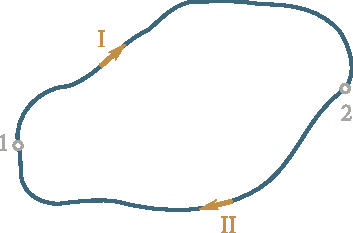
\includegraphics[scale=0.92]{figures/ch_03/fig_3_5.pdf}
			\caption[]{}
			\label{fig:3_5}
		\end{center}
	\end{minipage}
	\hspace{-0.05cm}
	\begin{minipage}[t]{0.5\linewidth}
		\begin{center}
			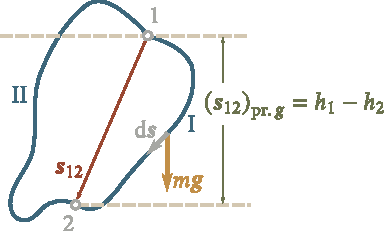
\includegraphics[scale=0.9]{figures/ch_03/fig_3_6.pdf}
			\caption[]{}
			\label{fig:3_6}
		\end{center}
	\end{minipage}
\end{figure}

Ta chứng tỏ rằng trọng lực là lực bảo toàn. Lực này tại mọi điểm đều có cùng độ lớn và cùng hướng nghĩa là hướng xuống dưới theo đường thẳng đứng (\fig{3_6}). Do đó, không phụ thuộc vào điều là hạt chuyển động theo quãng đường nào (chằng hạn I hoặc II, xem hình vẽ), công $A_{12}$ theo~\eqref{eq:3.19} được xác định bằng biểu thức 

\begin{equation*}
A_{12} = m\,(\vecdot{g}{s}_{12}) = mg(s_{12})_{\text{pr. }\vec{g}}.
\end{equation*}

\noindent
Từ \fig{3_6} rõ ràng là hình chiếu của vector $\vec{s}_{12}$ lên hướng $\vec{g}$ bằng hiệu các độ cao $h_1-h_2$. Do đó có thể viết biểu thức đối với công dưới dạng  
\begin{equation}\label{eq:3_23}
A_{12} = mg(h_1-h_2).
\end{equation}

\noindent
Biểu thức này rõ rằng không phụ thuộc vào quãng đường, từ đó suy ra trọng lực là lực bảo toàn.

Dễ dàng thu được cùng một kết quả cho bất kỳ trường đồng nhất tĩnh.

\begin{figure}[!htb]
	\begin{center}
		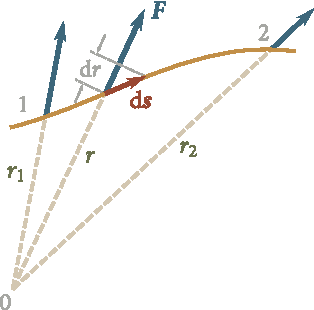
\includegraphics[scale=1]{figures/ch_03/fig_3_7.pdf}
		\caption[]{}
		\label{fig:3_7}
	\end{center}
\end{figure}

Các lực tác dụng lên hạt trong trường xuyên tâm cũng là các lực bảo toàn. Theo~ công thức \eqref{eq:3-18} công nguyên tố trên quãng đường $\deriv{s}$ (\fig{3_7}) bằng
\begin{equation*}
\deriv{A} = F(r)\,\deriv{s_F}.
\end{equation*}

\noindent
Nhưng hình chiếu của $\deriv{s}$ lên hướng của lực tại vị trí cho, nghĩa là lên hướng của bán kính vector $\vec{r}$, là bằng $\deriv{r}$ nghĩa là số gia của khoảng cách của hạt tính từ tâm lực O, $\deriv{s_F}=\deriv{r}$. Do đó $\deriv{A}=F(r)\,\deriv{r}$, còn công trên toàn quãng đường 
\begin{equation}\label{eq:3_24}
A_{12} = \int_{r_1}^{r_2} F(r)\,\deriv{r}.
\end{equation}

\noindent
Biểu thức này chỉ phụ thuộc vào dạng của hàm \eqref{eq:3_24} và vào các giá trị $r_1$ và $r_2$. Nó hoàn toàn không phụ thuộc vào dạng của quỹ đạo, từ đây suy ra rằng các lực là bảo toàn. 

Để không nảy sinh quan niệm sai ở độc giả là: mọi lực chỉ phụ thuộc vào tọa độ của điểm đều bảo toàn, ta hãy xét ví dụ sau. Giả sử các thành phần của lực được xác định bởi các công thức
\begin{equation}\label{eq:3_25}
F_x = ay,\quad F_y = -ax,\quad F_z=0.
\end{equation}

\begin{figure}[!htb]
	\begin{center}
		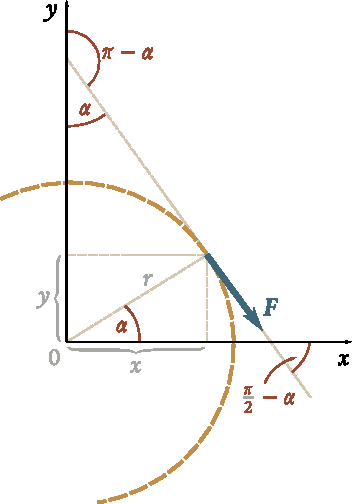
\includegraphics[scale=0.95]{figures/ch_03/fig_3_8.pdf}
		\caption[]{}
		\label{fig:3_8}
	\end{center}
\end{figure}

\noindent
Lực này có module bằng $F=ar$ và hướng theo tiếp tuyến của đường tròn bán kính $r$ (\fig{3_8}). Thật vậy, từ hình vẽ, ta thấy một lực có độ lớn và hướng 
\begin{align*}
F_x &= ar\cos\left(\frac{\pi}{2}-\alpha\right) = ar\sin\alpha = ar\,\frac{y}{r} = ay,\\
F_y &= ar\cos(\pi-\alpha) = ar\cos\alpha = -ar\,\frac{x}{r} = -ax,
\end{align*}

\noindent
sẽ có các thành phần trùng với các giá trị ~\eqref{eq:3_25}. Ta lấy một đường kín có dạng một đường tròn bán kính $r$ với tâm ở gốc tạo độ. Công của lực trên quãng đường này rõ rằng là bằng $F\times 2\pi r=ar\times 2\pi r=2\pi ar^2$, nghĩa là khác không. Do đó lực là không bảo toàn.

 Các lực ma sát là những lực điển hình không bảo toàn. Vì lực ma sát $\vec{F}$ và vân tốc $\vec{v}$ của hạt có chiều ngược nhau\footnote{Ở đây muốn nói đến trường hợp ma sát giữa một vật chuyển động và các vật đứng yên (đối với hệ quy chiếu). Trong một số trường hợp công của lực ma sát có thể dương. Điều này xảy ra, chẳng hạn, khi lực ma sát sinh ra bởi sự tương tác của một vật đã cho với một vất khác chuyển động  theo cùng một hướng nhưng với một vận tốc lớn hơn.} nên công của lực ma sát trên mỗi phần của quãng đường là âm:
\begin{equation*}
\deriv{A} = \vec{F}\,\deriv{\vec{s}} = (\vecdot{F}{v})\,\deriv{t} = -Fv\,\deriv{t} = -F\,\deriv{s}<0.
\end{equation*}

\noindent
Do đó công trên quãng đường kín bất kỳ sẽ âm (tức là khác không). Từ đó suy ra rằng các lực ma sát đều không bảo toàn.

Ta nhận thấy rằng, trường lực bảo toàn là một trường hợp riêng của trường thế. Trường lực được gọi là \textbf{trường thế}, nếu có thể mô tả trường nhờ hàm $V(x,y,z)$, mà gradient của nó (xem mục sau, \eqn{3_31}) xác định lực tại mỗi điểm của trường: $\vec{F}=\nabla V$ (so sánh với~\eqref{eq:3_32}). Hàm $V$ được gọi là \textbf{hàm thế} hoặc \textbf{thế vị}.

Trong trường hợp khi thế vị không phụ thuộc tường minh vào thời gian, tức là $V=V(x,y,z)$, thì trường thế là trường dừng, còn các lực của nó là các lực bảo toàn. Trong trường hợp đó: 


\begin{equation*}
V(x,y,z) = -E_{\text{p}}(x,y,z)
\end{equation*}

\noindent
trong đó $E_{\text{p}}(x,y,z)$ là thế năng của hạt (xem mục sau).

Đối với trường lực không dừng được mô tả bởi thế $V(x,y,z,t)$, không thể đồng nhất các lực thế và các lực bảo toàn với nhau.

\section{Thế năng trong trường lực ngoài}\label{sec:3_5}

Trong trường hợp khi công của các lực của trường không phụ thuộc vào quãng đường mà chỉ phụ thuộc vào các vị trí đầu và cuối của hạt thì ứng với mỗi điểm của trường có thể gán một giá trị của một hàm $E_{\text{p}}(x,y,z)$ nào đó sao cho hiệu các giá trị của hàm đó tại các điểm  $1$ và $2$ sẽ xác định công của các lực khi dịch chuyển hạt từ điểm đầu đến điểm thứ hai:
\begin{equation}\label{eq:3_26}
A_{12} = E_{\text{p},1} - E_{\text{p},2}.
\end{equation}

Sự so sánh này có thể tiến hành như sau. Tại điểm xuất phát $O$ nào đó ta viết giá trị tuỳ ý của hàm bằng  $E_{\text{p},0}$. Tại điểm $P$ tuỳ ý ta viết giá trị
\begin{equation}\label{eq:3_27}
E_{\text{p}}(P) = E_{\text{p},0} + A_{\text{p},0}
\end{equation}

\noindent
trong đó $A_{\text{p},0}$ là công được thực hiện trên hạt bởi các lực bảo toàn khi dịch chuyển hạt từ điểm $P$ đến điểm $0$. Vì công không phụ thuộc vào quãng đường nên giá trị $E_{\text{p}}(P)$ được xác định bằng cách như vậy sẽ là duy nhất. ta nhận hàm $E_{\text{p}}(P)$ có thứ nguyên của công (hoặc của năng lượng).

Theo \eqref{eq:3_27}, các giá trị của hàm tại các điểm $1$ và $2$ sẽ bằng 
\begin{equation*}
E_{\text{p},1} = E_{\text{p},0} + A_{10},\quad E_{\text{p},2} = E_{\text{p},0} + A_{20}.
\end{equation*}

\noindent
Ta lập hiệu của các giá trị đó và đồng thời lưu ý rằng $A_{20}=-A_{02}$ (xem mục trước). Kết quả là ta có
\begin{equation*}
E_{\text{p},1} - E_{\text{p},2} = A_{10} - A_{20} = A_{10} + A_{02}.
\end{equation*}

\noindent
Tổng $A_{10}+A_{02}$ cho công thực hiện bởi các lực của trường khi dịch chuyển hạt từ điểm $1$ đến điểm $2$ theo quỹ đạo đi qua điểm $0$. Tuy nhiên, công được thực hiện trên hạt khi dịch chuyển nó từ điểm $1$ đến điểm $2$ theo quỹ đạo khác bất kỳ (trong số đó có cả những quỹ đạo không đi qua điểm $0$) cũng sẽ  hệt như vậy. Do đó có thể viết tổng $A_{10}+A_{02}$ một cách đơn giản dưới dạng $A_{12}$. Tóm lại, ta có hệ thức \eqref{eq:3_26}.

Như vậy, nhờ hàm $E_{\text{p}}$ có thể xác định công được thực hiện trên hạt bởi các lực bảo toàn trên quãng đường bất kỳ, bắt đầu tại điểm tuỳ ý $1$ và kết thúc tại điểm tuỳ ý $2$.

Giả sử trên hạt chỉ có các lực bảo toàn tác dụng. Khi đó công được thực hiện trên hạt, trên quãng đường $1$-$2$ có thể được biểu thị dưới dạng \eqref{eq:3_26}. Theo công thức \eqref{eq:3_11}, công này chuyển thành số gia của động năng của hạt. Như vậy, ta đi tới đẳng thức
\begin{equation*}
E_{\text{k},2} - E_{\text{k},1} = E_{\text{p},1} - E_{\text{p},2}
\end{equation*}

\noindent
Từ đó suy ra rằng
\begin{equation*}
E_{\text{k},2} + E_{\text{p},2} = E_{\text{k},1} + E_{\text{p},1}
\end{equation*}

\noindent
Kết quả thu được có nghĩa là đại lượng 
\begin{equation}\label{eq:3_28}
E = E_{\text{k}} + E_{\text{p}}
\end{equation}

\noindent
đối với hạt nằm trong trường các lực bảo toàn là không đổi, tức là một tích phân chuyển động.

Từ \eqref{eq:3_28} suy ra $E_{\text{p}}$ tham gia vào tích phân chuyển động như một số hạng có thử nguyên của năng lượng. Do đó người ta gọi hàm $E_{\text{p}}(x,y,z)$ là  \textbf{thế năng} của hạt trong trường lực ngoài. Người ta gọi đại lượng  $E$ bằng tổng động năng và thế năng của hạt là \textbf{cơ năng toàn phần} của hạt.

Theo \eqref{eq:3_26}, công do các lực bảo toàn thực hiện trên hạt bằng độ giảm thế năng của hạt. Có thể nói một cách khác rằng công được thực hiện nhờ dự trữ thế năng.  

Từ \eqref{eq:3_27} suy ra rằng thế năng được xác định chính xác đến một hằng số cộng chưa biết nào đó $E_{\text{p},0}$. Tuy nhiên điều đó không có một ý nghĩa nào vì tham gia vào mọi hệ thức vật lý chỉ có hoặc hiệu các giá trị của $E_{\text{p}}$ tại hai vị trí của vật hoặc đạo hàm của hàm $E_{\text{p}}$ theo toạ độ thôi. Trên thực tế người ta quy ước coi thế năng của vật tại một vị trí nào đó là bằng không, còn lấy năng lượng tại các vị trí khác đối chiếu với năng lượng đó. 
Khi biết dạng của hàm $E_{\text{p}}(x,y,z)$, có thể tìm lực tác dụng lên hạt tại mỗi điểm của trường. Ta hãy xét sự dịch chuyển của một hạt song song với trục $x$ một lượng $\deriv{x}$. Sự dịch chuyển đó kéo theo sự thực hiện trên hạt một công bằng $\deriv{A}=\vec{F}\,\deriv{\vec{s}}=F_x\,\deriv{x}$ (các thành phần dịch chuyển $\deriv{y}$ và $\deriv{z}$ đều bằng không). Theo \eqref{eq:3_26}, công đó có thể được biểu thị như độ giảm thế năng: $\deriv{A}=-\deriv{E_{\text{p}}}$. So sánh cả hai biểu thức đối với công, ta có
\begin{equation*}
F_x\,\deriv{x} = -\deriv{E_{\text{p}}}
\end{equation*}

\noindent
Từ đó
\begin{equation*}
F_x = -\diff{E_{\text{p}}}{x}\, (y=\text{const},\, z=\text{const}).
\end{equation*}

\noindent
Biểu thức ở vế phải là đạo hàm $E_{\text{p}}(x,y,z)$ được tính với giả thiết các biến $y$ và $z$ là không biến thiên mà chỉ một biến $x$ biến thiên. Các đạo hàm tương tự được gọi là các đạo hàm riêng và được ký hiệu khác với $\diffinpartial{E_{\text{p}}}{x}$. Do đó thành phần của lực theo trục $x$ bằng đạo hàm riêng của thế năng theo biến $x$ được lấy với dấu ngược lại: $F_x=-\diffinpartial{E_{\text{p}}}{x}$. Đối với các thành phần của lực theo các trục  $y$ và $z$ có các biểu thức tương tự. Như vậy
\begin{equation}\label{eq:3_29}
F_x = -\diffpartial{E_{\text{p}}}{x},\quad F_y = -\diffpartial{E_{\text{p}}}{y},\quad F_z = -\diffpartial{E_{\text{p}}}{z}.
\end{equation}

Khi biết các thành phần có thể tìm được vector lực:
\begin{equation}\label{eq:3_30}
\vec{F} = F_x\vecuni{x} + F_y\vecuni{y} + F_z\vecuni{z} =
-\diffpartial{E_{\text{p}}}{x}\vecuni{x} - \diffpartial{E_{\text{p}}}{y}\vecuni{y} -\diffpartial{E_{\text{p}}}{z}\vecuni{z}.
\end{equation}

Vector với các thành phần $\diffinpartial{\varphi}{x}$,  $\diffinpartial{\varphi}{y}$, $\diffinpartial{\varphi}{z}$, trong đó $\varphi$ là hàm vô hướng của các toạ độ  $x,y,z$, được gọi là gradient của hàm $\varphi$ và được ký hiệu là $\varphi$ hoặc $\nabla\varphi$ ($\nabla$ được gọi là  \textbf{toán tử nabla}). Từ định nghĩa gradient suy ra rằng
\begin{equation}\label{eq:3_31}
\nabla\varphi = \diffpartial{\varphi}{x}\vecuni{x} + \diffpartial{\varphi}{y}\vecuni{y} + \diffpartial{\varphi}{z}\vecuni{z}.
\end{equation}

Sự so sánh ~\eqref{eq:3_30} với~\eqref{eq:3_31} chứng tỏ rằng lực bảo toàn bằng gradient của thế năng lấy với dấu ngược lại:
\begin{equation}\label{eq:3_32}
\vec{F} = -\nabla E_{\text{p}}.
\end{equation}

Giả sử rằng hạt dưới tác dụng của lực ~\eqref{eq:3_32} dịch chuyển được một đoạn $\deriv{\vec{s}}$ có các thành phần $\deriv{x}$, $\deriv{y}$, $\deriv{z}$. Đồng thời lực thực hiện một công 
\begin{equation*}
\deriv{A} = \vec{F}\,\deriv{\vec{s}} = -\nabla E_{\text{p}}\,\deriv{\vec{s}} = - \left(\diffpartial{E_{\text{p}}}{x}\,\deriv{x} + \diffpartial{E_{\text{p}}}{y}\,\deriv{y} +  \diffpartial{E_{\text{p}}}{z}\,\deriv{z}\right).
\end{equation*}

\noindent
Để ý rằng $\deriv{A}=-\deriv{E_{\text{p}}}$, đối với số gia của hàm $E_{\text{p}}$ ta có biểu thức sau:
\begin{equation}\label{eq:3_33}
\deriv{E_{\text{p}}} = \diffpartial{E_{\text{p}}}{x}\,\deriv{x} + \diffpartial{E_{\text{p}}}{y}\,\deriv{y} +  \diffpartial{E_{\text{p}}}{z}\,\deriv{z}.
\end{equation}

\noindent
Biếu thức dạng \eqref{eq:3_33} được gọi là vi phân toàn phần của hàm tương ứng.

Khái niệm vi phân toàn phần đóng vai trò quan trọng trong vật lý. Vì vậy ta dành một dòng cho nó. \textbf{Vi phân toàn phần} của một hàm đơn trị $f(x,y,z)$ là số gia của hàm đó có được khi chuyển từ điểm với các toạ độ $x,y,z$ đến điểm lân cận với các toạ độ $x+\deriv{x}, y+\deriv{y}, z+\deriv{z}$. Theo định nghĩa, số gia đó bằng
\begin{equation*}
\deriv{f}(x,y,z) = f(x+\deriv{x}, y+\deriv{y}, z+\deriv{z}) - f(x,y,z)
\end{equation*}

\noindent
và do đó chỉ được xác định bởi các giá trị của hàm tại các điểm đầu và cuối. Vì vậy nó không thể phụ thuộc vào quãng đường theo đó sự dịch chuyển xảy ra. Để làm quãng đường đó ta lấy một đường gấp khúc gồm các đoạn $\deriv{x}, \deriv{y}, \deriv{z}$ (\fig{3_9}). Trên đoạn $\deriv{x}v$, hàm $f(x,y,z)$ thể hiện như hàm của chỉ một biến $x$, và nhận số gia $(\diffinpartial{f}{x})\,\deriv{x}$. Tương tự, trên các đoạn $\deriv{y}$ và $\deriv{z}$, hàm nhận các số gia $(\diffinpartial{f}{y})\,\deriv{y}$ và $(\diffinpartial{f}{z})\,\deriv{z}$. Như vậy, số gia toàn phần của hàm khi dịch chuyển từ điểm đầu đến điểm cuối bằng 
\begin{equation}\label{eq:3_34}
\deriv{f}(x,y,z)  = \diffpartial{f}{x}\,\deriv{x} + \diffpartial{f}{y}\,\deriv{y} +  \diffpartial{f}{z}\,\deriv{z}.
\end{equation}

\noindent
Ta đã đi tới biểu thức đối với vi phân toàn phần (so sánh với  \eqref{eq:3_33}).

\begin{figure}[!htb]
	\begin{center}
		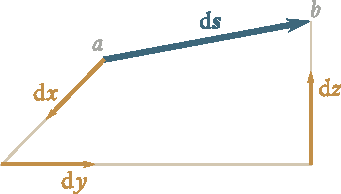
\includegraphics[scale=0.95]{figures/ch_03/fig_3_9.pdf}
		\caption[]{}
		\label{fig:3_9}
	\end{center}
\end{figure}

Không phải một biểu thức bất kỳ dạng
\begin{equation*}
P(x,y,z)\deriv{x} + Q(x,y,z)\deriv{y} + R(x,y,z)\deriv{z}
\end{equation*}

\noindent
cũng là vi phân toàn phần của hàm $f(x,y,z)$. Cụ thể là biểu thức đối với công được thực hiện bởi lực ~\eqref{eq:3_25}
\begin{equation}\label{eq:3_35}
\deriv{A} = ay\,\deriv{x} - ax\,\deriv{y}
\end{equation}

\noindent
không phải là vi phân toàn phần, nghĩa là không tồn tại một hàm $E_{\text{p}}$ mà  $-\diffinpartial{E_{\text{p}}}{x}=ay$, và $-\diffinpartial{E_{\text{p}}}{y}=-ax$ (xem ~\eqref{eq:3_25}). Một cách tương ứng, sẽ không tồn tại một hàm $E_{\text{p}}$ , mà độ giảm của nó đã có thể xác định được công ~\eqref{eq:3_35}.

Từ điều đã nêu suy ra rằng các lực bảo toàn chỉ có thể là các lực thoả mãn điều kiện ~\eqref{eq:3_32}, tức là các lực có các thành phần theo các trục toạ độ bằng các đạo hàm riêng của một hàm  $E_{\text{p}}(x,y,z)$ nào đó theo các toạ độ tương ứng, lấy với dấu ngoặc lại. Hàm đó là thế năng của hạt. 
Dạng cụ thể của hàm $E_{\text{p}}(x,y,z)$ phụ thuộc vào tính chất của trường lực. Để làm thí dụ ta tìm thế năng của hạt trong trọng trường. Theo \eqref{eq:3_23}, công được thực hiện trên hạt bởi các lực của trường đó bằng 
\begin{equation*}
A_{12} = mg(h_1-h_2).
\end{equation*}

\noindent
Mặt khác, theo \eqref{eq:3_26},
\begin{equation*}
A_{12} = E_{\text{p},1} - E_{\text{p},2}.
\end{equation*}

\noindent
So sánh cả hai biểu thức đối với công ta đi đến kết luận là thế năng của hạt trong trọng trường được xác định bằng biểu thức    
\begin{equation}\label{eq:3_36}
E_{\text{p}} = mgh
\end{equation}

\noindent
trong đó $h$ được tính từ một mức tuỳ ý.

Có thể chọn gốc tính thế năng một cách tuỳ ý. Do đó $E_{\text{p}}$ có thể có các giá trị âm. Chẳng hạn, nếu thừa nhận thế năng của hạt nằm tại mặt đất bằng không thì thế năng của hạt nằm tại đáy giếng có độ sâu $h'$ sẽ bằng $E_{\text{p}}=-mgh'$ (\fig{3_10}). Ta lưu ý rằng động năng không thể âm. 

\begin{figure}[!htb]
	\begin{center}
		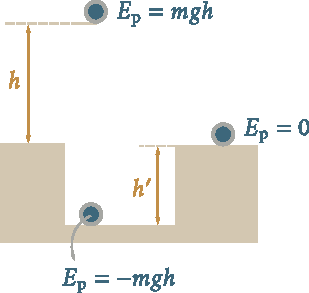
\includegraphics[scale=1]{figures/ch_03/fig_3_10.pdf}
		\caption[]{}
		\label{fig:3_10}
	\end{center}
\end{figure}

Giả sử ngoài các lực bảo toàn còn có một lực không bảo toàn $\vec{F}^*$ tác dụng lên hạt. Khi đó với sự dịch chuyển của hạt từ điểm $1$ đến điểm $2$, công sẽ được thực hiện trên hạt là 
\begin{equation*}
A_{12} = \int_{1}^{2} \vec{F}\,\deriv{\vec{s}} + \int_{1}^{2} \vec{F}^*\,\deriv{\vec{s}} = A_{\text{cons}} + A_{12}^*
\end{equation*}

\noindent
trong đó  $A_{12}^*$ là công của lực không bảo toàn. Có thể biểu diễn công của các lực bảo toàn $A_{\text{cons}}$ như $E_{\text{p},1}-E_{\text{p},2}$. Kết quả ta có:
\begin{equation*}
A_{12} = E_{\text{p},1} - E_{\text{p},2} + A_{12}^*
\end{equation*}
\noindent
Công tổng cộng của tất cả các lực đặt lên hạt chuyển thành độ tăng động năng của hạt (xem \eqref{eq:3_11}). Do đó,
\begin{equation*}
E_{\text{k},2} - E_{\text{p},1} = E_{\text{p},1} - E_{\text{p},2} + A_{12}^*
\end{equation*}

\noindent
từ đó, để ý rằng  $E_{\text{k}}+E_{\text{p}}=E$, ta có
\begin{equation}\label{eq:3_37}
E_2 - E_1 = A_{12}^*.
\end{equation}

\noindent
Kết quả nhận được có nghĩa là công của các lực không bảo toàn chỉ được dùng để gia tăng cơ năng toàn phần của hạt. 

Trong trường hợp nếu tại các vị trí đầu và cuối động năng của hạt như nhau (cụ thể bằng không ), thì công của các lực không bảo toàn chuyển thành độ tăng thế năng của hạt:
\begin{equation}\label{eq:3_38}
A_{12}^* = E_{\text{p},2} - E_{\text{p},1}
\end{equation}

\noindent
($E_{\text{k},2}=E_{\text{k},1}$). Hệ thức đặc biệt này thuận tiện khi tìm hiệu các giá trị của thế năng. 

Ta xét hệ gồm $N$ hạt không tương tác lẫn nhau nằm trong trường các lực bảo toàn. Mỗi hạt có động năng $E_{\text{k},i}=m_iv_i^2/2$ ($i$ là số thứ tự của hạt) và thế năng $E_{\text{p},i}=E_{\text{p},i}(x_i,y_i,z_i)$. Nếu xét hạt thứ $i$ độc lập với các hạt khác thì có thể thu được
\begin{equation*}
E_i = E_{\text{k},i} + E_{\text{p},i} = \text{constant}_i
\end{equation*}

\noindent
Lấy tổng đẳng thức đó theo tất cả các hạt, ta đi đến hệ thức
\begin{equation}\label{eq:3_39}
E = \sum_{i=1}^{N}E_i = \sum_{i=1}^{N}E_{\text{k},i} + \sum_{i=1}^{N}E_{\text{p},i} = \text{constant}.
\end{equation}

\noindent
Từ hệ thức này suy ra tính cộng được của cơ năng toàn phần đối với hệ đang xét.
Theo \eqref{eq:3_39}, \textit{cơ năng toàn phần của hệ các hạt không tương tác lẫn nhau mà chỉ có các lực bảo toàn tác dụng lên chúng là không đổi}. Điều khẳng định này biểu thị định luật bảo toàn năng lượng đối với hệ cơ học đã nêu.

Nếu ngoài các lực bảo toàn còn các lực không bảo toàn tác dụng lên hạt thì năng lượng toàn phần của hệ sẽ biến đổi, đồng thời
\begin{equation}\label{eq:3_40}
E_2 - E_1 = \sum_{i=1}^{N}(A_{12}^*)_i
\end{equation}

\noindent
trong đó $(A_{12}^*)_i$ là công được thực hiện bởi các lực không bảo toàn đặt lên hạt thứ $i$ khi dịch chuyển hạt này từ vị trí đầu đến vị trí cuối.

Trong đoạn cuối của mục trước ta đã thiết lập rằng công của lực ma sát luôn luôn là âm. Do đó nếu có các lực ma sát trong hệ thì cơ năng toàn phần của hệ bị giảm (bị tiêu tán), chuyển thành các dạng năng lượng không cơ học (chẳng hạn, thành nội năng của các vật hoặc như thường nói, thành nhiệt). Quá trình đó được gọi là \textbf{sự tiêu tán năng lương} (thuật ngữ latin ``dissipatio`` có nghĩa là sự tiêu tán). Các lực dẫn đén sự tiêu tán năng lượng được gọi là lực tiêu tán. Như vậy, các lực ma sát là các  \textbf{lực tiêu tán}. Trong trường hợp tổng quát các lực tiêu tán là các lực luôn luôn hướng ngược chiều với vận tốc của hạt, và do đó gây ra sự hãm chúng. 

Ta hãy lưu ý rằng các lực không bảo toàn không nhất thiết phải là các lực tiêu tán.

\section{Thế năng tương tác}\label{sec:3_6}

Cho đến nay ta đã nghiên cứu hệ các hạt không tương tác lẫn nhau. Bây giờ ta chuyển sang xét hệ gồm hai hạt tương tác lẫn nhau. Ta ký hiệu lực mà hạt thứ hai tác dụng lên hạt thứ nhất bằng $\vec{F}_{12}$, còn lực mà hạt thứ nhất tác dụng lên hạt thứ hai bằng $\vec{F}_{21}$. Theo định luật Newton thứ ba $\vec{F}_{12}=-\vec{F}_{21}$.

Ta đưa vào vector $\vec{R}_{12}=\vec{r}_2-\vec{r}_1$ , trong đó $\vec{r}_1$ và $\vec{r}_2$ là các bán kính vector của các hạt (\fig{3_11}). Giả sử rằng các lực $\vec{F}_{12}$ và $\vec{F}_{21}$ có độ lớn chỉ phụ thuộc vào khoảng cách $\vec{R}_12$ giữa các hạt và hướng dọc theo đường thẳng nối các hạt. Điều đó, như ta đã biết, đúng dối với các lực lượng tương tác hấp dẫn và Coulomb (xem các công thức~\eqref{eq:2_18} và~\eqref{eq:2_23}).

Với các giả thiết đã cho có thể viết các lực $\vec{F}_{12}$ và $\vec{F}_{21}$ dưới dạng 

\begin{equation}\label{eq:3_41}
\vec{F}_{12} = -\vec{F}_{21} = f(R_{12})\vecuni{12}
\end{equation}

\noindent
trong đó $\vecuni{12}$ là chuẩn của vector $\vec{R}_{12}$ (\fig{3_12}), còn $f(R_{12})$ là một hàm nào đó của $R_{12}$, dương trong trường hợp các hạt hút lẫn nhau và âm trong trường hợp chúng đẩy nhau.

Coi hệ là kín (không có các ngoại lực), ta viết phương trình chuyển động của cả hai hạt:

\begin{equation*}
m_1\dot{\vec{v}}_1 = \vec{F}_{12},\quad m_2\dot{\vec{v}}_2 = \vec{F}_{21}
\end{equation*}

\noindent
Nhân phương trình đầu với $\deriv{\vec{r}_1}=\vec{v}_1\,\deriv{t}$, phương trình thứ hai với $\deriv{\vec{r}_2}=\vec{v}_2\,\deriv{t}$ và cộng chúng lại\footnote{Trong trường hợp đã cho hãy ký hiệu một cách hợp lý dịch chuyển hạt qua $\deriv{\vec{r}}$ thay cho $\deriv{\vec{s}}$.}. Kết quả ta có hệ thức
\begin{equation}\label{eq:3_42}
m_1\vec{v}_1\dot{\vec{v}}_1\,\deriv{t} + m_2\vec{v}_2\dot{\vec{v}}_2\,\deriv{t} = \vec{F}_{12}\,\deriv{\vec{r}_1} + \vec{F}_{21}\,\deriv{\vec{r}_2}.
\end{equation}

\begin{figure}[!htb]
	\begin{minipage}[t]{0.5\linewidth}
		\begin{center}
			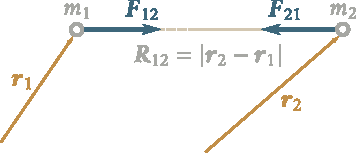
\includegraphics[scale=0.89]{figures/ch_03/fig_3_11.pdf}
			\caption[]{}
			\label{fig:3_11}
		\end{center}
	\end{minipage}
	\hspace{-0.05cm}
	\begin{minipage}[t]{0.5\linewidth}
		\begin{center}
			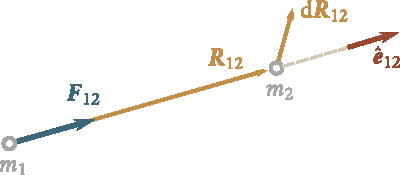
\includegraphics[scale=0.89]{figures/ch_03/fig_3_12.pdf}
			\caption[]{}
			\label{fig:3_12}
		\end{center}
	\end{minipage}
\end{figure}

\noindent
Vế trái của hệ thức này là độ tăng động năng của hệ trong khoảng thời gian $\deriv{t}$ (xem \eqref{eq:3_3}), vế phải là công của các nội lực trong cùng khoảng thời đó.
Để ý đến biểu thức ~\eqref{eq:3_41} có thể biến đổi vế phải của công thức \eqref{eq:3_42} như sau:
\begin{equation}\label{eq:3_43}
\deriv{A}_{\text{int}} = \vec{F}_{12}\,\deriv{\vec{r}_1} + \vec{F}_{21}\,\deriv{\vec{r}_2} = -\vec{F}_{12}\,\deriv{(\vec{r}_2-\vec{r}_1)} = -\vec{F}_{12}\,\deriv{\vec{R}_{12}}.
\end{equation}

\noindent
Theo \eqref{eq:3_41}, thế $\vec{F}_{12}$ vào biểu thức trên, ta được 
\begin{equation*}
\deriv{A}_{\text{int}} = - f(R_{12}) \vecuni{12} \, \deriv{\vec{R}_{12}}.
\end{equation*}

\noindent
Từ \fig{3_12} rõ ràng là tích vô hướng $\vecuni{12}\,\deriv{\vec{R}_{12}}$ sẽ bằng $\deriv{R_{12}}$ là số gia của khoảng cách giữa các hạt. Như vậy
\begin{equation}\label{eq:3_44}
\deriv{A}_{\text{int}} = - f(R_{12})\,\deriv{R_{12}}.
\end{equation}

%\begin{figure}[t]
%	\begin{center}
%		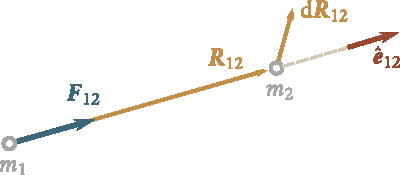
\includegraphics[scale=1]{figures/ch_03/fig_3_12.pdf}
%		\caption[]{}
%		\label{fig:3_12}
%	\end{center}
%%	\vspace{-0.7cm}
%\end{figure}

Có thể coi biểu thức $f(R_{12})\,\deriv{R_{12}}$  như là số gia của một hàm nào đó của $R_{12}$. Ký hiệu hàm này bằng $E_{\text{p}}(R_{12})$, ta đi đến đẳng thức:
\begin{equation}\label{eq:3_45}
f(R_{12})\,\deriv{R_{12}} = \deriv{E_{\text{p}}(R_{12})}.
\end{equation}

\noindent
Do đó
\begin{equation}\label{eq:3_46}
\deriv{A}_{\text{int}} = \deriv{E_{\text{p}}}.
\end{equation}

 Để ý đến toàn bộ điều đã nêu có thể viết biểu thức \eqn{3_42} dưới dạng $\deriv{E_{\text{k}}}=-\deriv{E_{\text{p}}}$, hoặc
\begin{equation}\label{eq:3_47}
\deriv{E} = \deriv{(E_{\text{k}}+E_{\text{p}})} = 0
\end{equation}

\noindent
từ đó suy ra rằng đại lượng $E=E_{\text{k}}+E_{\text{p}}$ đối với hệ kín là đang xét được bảo toàn. Hàm $E_{\text{p}}(R_{12})$ 
 là \textbf{thế năng tương tác}. Nó phụ thuộc vào khoảng cách giữa các hạt.

Giả sử cấc hạt đã dời khỏi các vị trí mà tại các vị trị này khoảng các giữa chúng bằng $R_{12}^{(a)}$, sang các vị trí mới mà tịa các vị trí đó khoảng cách giữa chúng bằng $R_{12}^{(b)}$. Theo \eqref{eq:3_46} các nội lực thực hiện đồng thời trên các hạt một công: 
\begin{equation}\label{eq:3_48}
A_{\text{ab, int}} = - \int_{a}^{b} \deriv{E_{\text{p}}} = E_{\text{p}}[R_{12}^{(a)}] - E_{\text{p}}[R_{12}^{(b)}].
\end{equation}

\noindent
Từ~\eqref{eq:3_48} suy rằng công của các lực~\eqref{eq:3_41} không phụ thuộc vào quãng đường theo đó các hạt dịch chuyển và chỉ được xác định bởi các khoảng các đầu và cuối giữa các hạt (bởi các cấu hình đầu và cuối của hệ). Như vậy các lực tương tác dạng~\eqref{eq:3_41} là các lực bảo toàn.

Nếu cả hai hạt đều chuyển động thì năng lượng toàn phần của hệ bằng 
\begin{equation}\label{eq:3_49}
E = \frac{m_1v_1^2}{2} + \frac{m_2v_2^2}{2} + E_{\text{p,ia}}(R_{12}) 
\end{equation}

\noindent
với $E_{\text{p,ia}}(R_{12})$ là thế năng tương tác.

Ta giả thiết rằng hạt $1$ được gắn cố định tại một điểm nào đó mà ta dùng làm gốc tọa độ ($\vec{r}_1=0$). Kết quả là hạt đó mất khả năng chuyển động, do đó động năng chỉ tạo thành từ một số hạng $m_2v_2^2/2$. Trong trường hợp này thế năng sẽ là hàm chỉ của $\vec{r}_2$. Vì vậy biểu thức~\eqref{eq:3_49} nhận dạng

\begin{equation}\label{eq:3_50}
E = \frac{m_2v_2^2}{2} + E_{\text{p,ia}}(r_2).
\end{equation}

\noindent
Nếu xét hệ chỉ gồm một hat $2$ thì hàm $E_{\text{p,ia}}$ sẽ đóng vai trò thế năng của hạt $2$ trong trường hợp các lực được tạo thành bởi hạt $1$. Tuy nhiên về thực chất hàm này là thế năng tương tác của hạt $1$ và hạt $2$. Nói chung, thế năng trong trường lực ngoài thực chất là năng lượng tương tấc giữa các vật của hệ và các vật tạo thành trường lực ngoài đối với hệ. 

Ta trở lại hệ gồm hai hạt tương tác tự do (``không cố định''). Nếu ngoài các nội lực ra, ngoại lực $\vec{F}_1^*$  tác dụng lên hạt thứ nhất, còn lực $\vec{F}_2^*$ tác dụng lên hạt thứ hai, thì các số hạng $\vec{F}_1^*\,\deriv{\vec{r}_1^*}$ và $\vec{F}_2^*\,\deriv{\vec{r}_2^*}$ tham gia vào vế phải của hệ thức~\eqref{eq:3_42} mà tổng của chúng cho công $\deriv{A_{\text{ext}}}$ của các ngoại lực. Tương ứng, công thức~\eqref{eq:3_47} nhận dạng  
\begin{equation}\label{eq:3_51}
\deriv{(E_{\text{k}}+E_{\text{p,ia}})} = \deriv{A_{\text{ext}}}.
\end{equation}
    
Trong trường hợp khi động năng tổng hợp của các hạt là không đổi (chẳng hạn, bằng không) hệ thức~\eqref{eq:3_51} có dạng như sau:
\begin{equation}\label{eq:3_52}
\deriv{E_{\text{p,ia}}} = \deriv{A_{\text{ext}}}
\end{equation}

\noindent
(ở đây $\deriv{E_{\text{k}}}=0$). Lấy tích phân hệ thức này từ cấu hình $a$ đến cấu hình $b$ ta có:
\begin{equation}\label{eq:3_53}
E_{\text{p,ia}}[R_{12}^{(b)}] - E_{\text{p,ia}}[R_{12}^{(a)}] = \deriv{A_{\text{ab,ext}}}
\end{equation}

\noindent
($E_{\text{k},b}=E_{\text{k},a}$) (so sánh với công thức~\eqref{eq:3_38}).

Ta hãy mở rộng các kết quả thu được cho hệ gồm ba hạt tương tác lẫn nhau, Trong trường hợp này công của các nội lực bằng
\begin{equation}\label{eq:3_54}
\deriv{A_{\text{int}}} = (\vec{F}_{12} + \vec{F}_{13})\,\deriv{\vec{r}_1} + (\vec{F}_{21} + \vec{F}_{23})\,\deriv{\vec{r}_2} + (\vec{F}_{31} + \vec{F}_{32})\,\deriv{\vec{r}_3}.
\end{equation}

\noindent
Để ý rằng $\vec{F}_{ik}=-\vec{F}_{ki}$ ta đưa biểu thức ~\eqref{eq:3_54} về dạng
\begin{align}
\deriv{A_{\text{int}}} &= - \vec{F}_{12}\,\deriv{(\vec{r}_2-\vec{r}_1)} - \vec{F}_{13}\,\deriv{(\vec{r}_3-\vec{r}_1)} - \vec{F}_{23}\,\deriv{(\vec{r}_3-\vec{r}_2)}\nonumber\\
&= - \vec{F}_{12}\,\deriv{\vec{R}_{12}} - \vec{F}_{13}\,\deriv{\vec{R}_{13}} - \vec{F}_{23}\,\deriv{\vec{R}_{23}}\label{eq:3_55}
\end{align}

\noindent
trong đó $\vec{R}_{ik}=\vec{r}_k-\vec{r}_i$.

Giả thiết rằng các nội lực có thể được biểu diễn dưới dạng $\vec{F}_{ik}=f_{ik}(R_{ik})\vecuni{ik}$ (so sánh với \eqref{eq:3_41}). Khi đó
\begin{equation*}
\deriv{A_{\text{int}}} = - f_{12}(R_{12})\vecuni{12}\,\deriv{\vec{R}_{12}} - f_{13}(R_{13})\vecuni{13}\,\deriv{\vec{R}_{13}} - f_{23}(R_{23})\vecuni{23}\,\deriv{\vec{R}_{23}}.
\end{equation*}

\noindent
Mỗi tích $\vecuni{ik}\,\deriv{R_{ik}}$ bằng số gia của khoảng cách giữa các hạt tương ứng  $\deriv{R_{ik}}$. Vì vậy
\begin{align}
\deriv{A_{\text{int}}} &= - f_{12}(R_{12})\,\deriv{R_{12}} - f_{13}(R_{13})\,\deriv{R_{13}} - f_{23}(R_{23})\,\deriv{R_{23}}\nonumber\\
&= - \deriv{[E_{\text{p},12}(R_{12}) + E_{\text{p},13}(R_{13}) + E_{\text{p},23}(R_{23})]} = - \deriv{E_{\text{p,ia}}}.\label{eq:3_56}
\end{align}

\noindent
Ở đây 
\begin{equation}\label{eq:3_57}
E_{\text{p,ia}} = E_{\text{p},12}(R_{12}) + E_{\text{p},13}(R_{13}) + E_{\text{p},23}(R_{23})
\end{equation}

\noindent
là \textbf{thế năng tương tác của hệ }. Nó được gộp từ các năng lượng tương tác của các hạt, lấy theo từng cặp. 

Đánh giá $\deriv{E_{\text{k}}}$ ngang với tổng các công $\deriv{A_{\text{int}}}=-\deriv{E_{\text{p,ia}}}$ và $\deriv{A_{\text{ext}}}$ ta đi đến hệ thức~\eqref{eq:3_51}, trong đó cần hiểu $E_{\text{p,ia}}$ là biểu thức~\eqref{eq:3_57}.

Dễ dàng tổng quát hóa kết quả thu được cho hệ gồm một số hạt bất kỳ. Đối với hệ gồm $N$ hạt tương tác với nhau thế năng tương tác được gộp từ các năng lượng tương tác của các hạt, lấy theo từng cặp:
\begin{multline}\label{eq:3_58}
E_{\text{p,ia}} = E_{\text{p},12}(R_{12}) + E_{\text{p},13}(R_{13}) + \ldots + E_{\text{p},1N}(R_{1N})\\
+ E_{\text{p},23}(R_{23}) + E_{\text{p},2N}(R_{2N}) + \ldots + E_{\text{p},N-1,N}(R_{N-1,N}).
\end{multline}

\noindent 
Có thể viết tổng  này như sau: 
\begin{equation}\label{eq:3_59}
E_{\text{p,ia}} = \sum_{i<k} E_{\text{p},ik}(R_{ik})
\end{equation}

\noindent 
(lưu ý rằng trong biểu thức~\eqref{eq:3_58}, ở mỗi số hạng chỉ số thứ nhất có giá trị bé hơn chỉ số thứ hai). Vì rằng $E_{\text{p},ik}(R_{ik})=E_{\text{p},ki}(R_{ki})$ nên cũng có thể biểu diễn năng lượng tương tác dưới dạng 
\begin{equation}\label{eq:3_60}
E_{\text{p,ia}} = \frac{1}{2}\,\sum_{i\neq k} E_{\text{p},ik}(R_{ik}).
\end{equation}

\noindent
Trong các tổng~\eqref{eq:3_59} và~\eqref{eq:3_60}, các chỉ số $i$ và $k$ lấy các giá trị từ 1 đến $N$,tuân theo điều kiện $i<k$ hoặc $i\neq k$.

Giả sử hệ gồm bốn hạt, trong đó hạt thứ nhất chỉ tương tác với hạt thứ hai và thứ ba chỉ tương tác với hạt thứ tư. Khi đó năng lượng toàn phần của hệ sẽ bằng 
\begin{align}
E &= E_{\text{k},1} + E_{\text{k},2} + E_{\text{k},3} + E_{\text{k},4} + E_{\text{k},12} + E_{\text{k},34}\nonumber\\
&= (E_{\text{k},1} + E_{\text{k},2} + E_{\text{k},12}) + (E_{\text{k},3} + E_{\text{k},4} + E_{\text{k},34}) = E' + E''. \label{eq:3_61}
\end{align}

\noindent
Ở đây $E'$ là năng lượng toàn phần của hệ con tạo nên bởi các hạt $1$ và $2$, và $E''$ là năng lượng toàn phần của hệ con tạo nên bởi các hạt $3$ và $4$. Theo giả thiết sự tương tác giữa các hệ con là không có. Hệ thức~\eqref{eq:3_61} chứng tỏ tính cộng được của năng lượng (xem đoạn thứ ba của~\ref{sec:3_1})

Để kết thúc ta tìm dạng hàm $E_{\text{p,ia}}$ trong trường hợp khi lực tương tác tỷ lệ nghịch với bình phương khoảng cách giữa các hạt: 
\begin{equation}\label{eq:3_62}
f(R_{12}) = \frac{\alpha}{R_{12}^2}
\end{equation}

\noindent
($\alpha$ là hằng số). Ta nhớ rằng trong trường hợp các hạt hút nhau s $\alpha>0$, trong trường hợp các hạt đẩy nhau $\alpha<0$ (xem đoạn sau công thức~\eqref{eq:3_41}).

Theo~\eqref{eq:3_45}
\begin{equation*}
\deriv{E_{\text{p,ia}}} = f(R_{12})\,\deriv{R_{12}} = \frac{\alpha}{R_{12}^2}\,\deriv{R_{12}}.
\end{equation*}

\noindent
Phép tích phân cho 
\begin{equation}\label{eq:3_63}
E_{\text{p,ia}} = - \frac{\alpha}{R_{12}} + \text{constant}.
\end{equation}

Hệt như thế năng trong trường lực ngoài, thế năng tương tác được xác định chính xác đến hằng số cộng tùy ý. Thông thường người ta giả thiết rằng với $R_{12}=\infty$ thế năng sẽ bị triệt tiêu (với khoảng cách đó lực~\eqref{eq:3_62} bị triệt tiêu nghĩa là sự tương tác giữa các hạt biến mất). Khi đó hằng số cộng trong~\eqn{3_63} trở thành bằng không và biểu thức đối với thế năng tương tác có dạng 
\begin{equation}\label{eq:3_64}
E_{\text{p,ia}} = - \frac{\alpha}{R_{12}}.
\end{equation}

Theo~\eqn{3_53} thì việc đẩy các hạt ra xa nhau từ khoảng cách $R_{12}$ đến khoảng cách lớn vô hạn, mà lại không thay đổi vận tốc của chúng, sẽ đòi hỏi phải thực hiện một công
\begin{equation*}
A_{\text{ext}} = E_{\text{p,ia}}(\infty) - E_{\text{p,ia}}(R_{12}).
\end{equation*}

\noindent
Phép thế các giá trị tương ứng của hàm~\eqref{eq:3_64} dẫn đến biểu thức
\begin{equation}\label{eq:3_65}
A_{\text{ext}} = 0 - \left(-\frac{\alpha}{R_{12}}\right) = \frac{\alpha}{R_{12}}.
\end{equation}

Trong trường hợp các hạt hút nhau $\alpha>0$; một cách thích ứng để đẩy các hạt ra xa nhau đòi hỏi thực hiện một công dương.

Trong trường hợp các hạt đẩy nhau $\alpha<0$ và công~\eqref{eq:3_65} là âm. Phải thực hiện công đó dễ ngăn cản các hạt đẩy nhau tăng vận tốc chuyển động của mình.

%\vspace{-12pt}

\section{Định luật bảo toàn năng lượng}\label{sec:3_7}

Ta hãy tổng hợp các kết quả thu được trong các tiết trước với nhau. Ta nghiên cứu hệ gồm $N$ hạt với các khối lượng $m_1, m_2, \ldots, m_N$. Giả thử các hạt tương tác lẫn nhau với các lực $\vec{F}_{ik}$ mà các module của chúng chỉ phụ thuộc vào khoảng cách $R_{ik}$ giữa các hạt. Trong tiết trước ta đã chứng minh rằng các lực như thế là các lực bảo toàn. Điều này có nghĩa là công do các lực này thực hiện trên các hạt được xác định bằng các cấu hình đầu và cuối của hệ. Ta giả thử rằng ngoài các nội lực còn có ngoại lực bảo toàn $\vec{F}_i$ và ngoại lực không bảo toàn $\vec{F}_i^*$ tác dụng lên hạt thứ $i$. Khi đó phương trình chuyển động của hạt thứ $i$ sẽ có dạng 
\begin{equation}\label{eq:3_66}
m_i\dot{\vec{v}}_i = \sum_{\substack{k=1\\(k\neq i)}}^{N} \vec{F}_{ik} + \vec{F}_i + \vec{F}_i^*
\end{equation}

\noindent
trong đó $i=1,2,\ldots,N$.

Nhân phương trình thứ $i$ với $\deriv{\vec{s}_i}=\deriv{\vec{r}_i}=\vec{v}_i\,\deriv{t}$ và cộng tất cả $N$ phương trình, ta có:
\begin{equation}\label{eq:3_67}
\sum_{i=1}^{N} m_i\vec{v}_i\,\deriv{\vec{v}_i} = \sum_{i=1}^{N}\left[\sum_{\substack{k=1\\(k\neq i)}}^{N} \vec{F}_{ik}\right]\,\deriv{\vec{r}_i} + \sum_{i=1}^{N}\vec{F}_i\,\deriv{\vec{s}_i} + \sum_{i=1}^{N}\vec{F}_i^*\,\deriv{\vec{s}_i}.
\end{equation}

\noindent
Vế trái là độ tăng động năng của hệ: 
\begin{equation}\label{eq:3_68}
\sum_{i=1}^{N} m_i\vec{v}_i\,\deriv{\vec{v}_i} = \deriv{\left[\sum_{i=1}^{N} \frac{m_iv_i^2}{2}\right]} = \deriv{E_{\text{k}}}
\end{equation}

\noindent
(xem \eqref{eq:3_3}). Từ các công thức ~\eqref{eq:3_54} và \eqref{eq:3_59} suy ra rằng số hạng thứ nhất của vế phải bằng độ giảm thế năng tương tác của các hạt:
\begin{equation}\label{eq:3_69}
\sum_{i=1}^{N}\left[\sum_{\substack{k=1\\(k\neq i)}}^{N} \vec{F}_{ik}\right]\,\deriv{\vec{r}_i} = - \sum_{i<k}\vec{F}_{ik}\,\deriv{\vec{R}_{ik}} = -\deriv{\left[\sum_{i<k} E_{\text{p},ik}(R_{ik})\right]} = -\deriv{E_{\text{p,ia}}}.
\end{equation}

\noindent
Theo \eqn{3_26}, số hạng thứ hai trong \eqn{3_67} bằng độ giảm thế năng của hệ trong trường ngoài của các lực bảo toàn: 
\begin{equation}\label{eq:3_70}
\sum_{i=1}^{N}\vec{F}_i\,\deriv{\vec{s}_i} = -\deriv{\left[\sum_{i=1}^{N}E_{\text{p},i}(\vec{r}_i)\right]} = -\deriv{E_{\text{p,ext}}}.
\end{equation}

\noindent
Cuối cùng, số hạng trong  \eqn{3_67} là công của các ngọai lực không bảo toàn:
\begin{equation}\label{eq:3_71}
\sum_{i=1}^{N}\vec{F}_i^*\,\deriv{\vec{s}_i} = \sum_{i=1}^{N} \deriv{A_i^*} = \deriv{A^*_{\text{ext}}}.
\end{equation}

\noindent
Chú ý đến các công thức ~\eqref{eq:3_68} và \eqref{eq:3_71}, ta biểu diễn biểu thức \eqref{eq:3_67} như sau: 
\begin{equation}\label{eq:3_72}
\deriv{(E_{\text{k}} + E_{\text{p,ia}} + E_{\text{p,ext}})} = \deriv{A^*_{\text{ext}}}.
\end{equation}

Đại lượng
\begin{equation}\label{eq:3_73}
E = E_{\text{k}} + E_{\text{p,ia}} + E_{\text{p,ext}}
\end{equation}

\noindent
là cơ năng toàn phần của hệ. Nếu các ngoại lực không bảo toàn không có mặt thì vế phải của công thức \eqref{eq:3_72} sẽ bằng không, và do đó năng lượng toàn phần của hệ là không đổi: 
\begin{equation}\label{eq:3_74}
E = E_{\text{k}} + E_{\text{p,ia}} + E_{\text{p,ext}} = \text{constant}.
\end{equation}

\noindent
Như vậy, ta đã đi tới kết luận là 
 \textit{cơ năng toàn phần của một hệ vật chỉ chịu tác dụng của các lực bảo toàn là không đổi}. Trong khẳng định này có chứa nội dung của một định luật cơ bản của cơ học đó là \textbf{định luật bảo toàn cơ năng}.

Đối với một hệ kín, nghĩa là trong đó không có một ngoại lực nào tác dụng lên các vật của hệ , hệ thức \eqref{eq:3_74} có dạng 
\begin{equation}\label{eq:3_75}
E = E_{\text{k}} + E_{\text{p,ia}} = \text{const}.
\end{equation}

\noindent
Trong trường hợp này định luật bảo toàn năng lượng được diễn đạt như sau: \textit{cơ năng toàn phần của một hệ vật kín mà giữa các vật này chỉ có lực bảo toàn tác dụng là không đổi}.

Nếu trong một hệ kín ngoài các lực bảo toàn còn có cả các lực không bảo toàn tác dụng, chẳng hạn các lực ma sát, thì cơ năng toàn phần của hệ sẽ không bảo toàn. Nếu coi các lực không bảo toàn như các ngoại lực, thì theo \eqn{3_72} có thể viết: 
\begin{equation}\label{eq:3_76}
\deriv{E} = \deriv{(E_{\text{k}} + E_{\text{p,ia}})} = \deriv{A_{\text{non-cons}}}.
\end{equation}

\noindent
Lấy tích phân hệ thức này ta có: 
\begin{equation}\label{eq:3_77}
E_2 - E_1 = A_{12,\text{non-cons}}.
\end{equation}

Định luật bảo toàn năng lượng đối với hệ các hạt không tương tác đã được phát biểu trong mục~\ref{sec:3_5} (xem đoạn sau công thức \eqref{eq:3_39}).

\section{Năng lượng biến dạng đàn hồi}\label{sec:3_8}

Không chỉ một hệ vật tương tác mà cả một vật biến dạng đàn hồi được lấy riêng rẽ (chẳng hạn, một lò xo bị nén, một thanh được kẽo dãn, v.v..) có thể có thế năng. Trong trường hợp này thế năng phụ thuộc vào vị trí tương hỗ của các phần riêng biệt của vật (chẳng hạn, vào khoảng cách giữa các vòng lò xo lân cận nhau).

Theo công thức~\eqref{eq:3_13}, cần tốn công $A=kx^2/2$ cho cả sự dãn ra lẫn sự nén lò xo lại một lượng $x$. Công này làm tăng thế năng của lò xo. Do đó, sự phụ thuộc của thế năng của lò xo vào độ dãn $x$ có dạng:
\begin{equation}\label{eq:3_78}
E_{\text{p}} = \frac{kx^2}{2}
\end{equation}

\noindent
trong đó $k$ là hệ số cứng của lò xo (xem mục~\ref{sec:2_9})). Công thức~\eqref{eq:3_78} được viết với giả thiếu là thế năng của lò xo chưa biến dạng là bằng không. Trên hình~\ref{fig:3_13} biểu diễn đồ thị của sự phụ thuộc của $E_{\text{p}}$ vào $x$. 

\begin{figure}[!htb]
	\begin{center}
		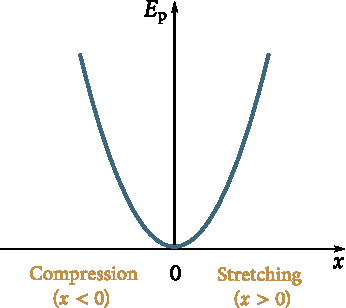
\includegraphics[scale=1]{figures/ch_03/fig_3_13.pdf}
		\caption[]{}
		\label{fig:3_13}
	\end{center}
\end{figure}

Với sự biến dạng đàn hồi theo chiều dọc của một thanh, công được xác định bởi công thức~\eqref{eq:3_14} sẽ được thực hiện. Theo đó thế năng của một thanh biến dạng đàn hồi là bằng
\begin{equation}\label{eq:3_79}
E_{\text{p}} = \frac{E\varepsilon^2}{2}\,V
\end{equation}

\noindent
Ở đây $E$ là suất Young, $\varepsilon$ là độ dãn tỷ đối và $V$ là thể tích của thanh.

Ta đưa vào sự khảo sát mật độ năng lượng biến dạng đàn hồi 

Let us introduce the concept of the density of the energy of elastic deformation $w_{\text{e}}$, which we shall define as the ratio of the energy $\deriv{E_{\text{p}}}$ to the volume $\deriv{V}$ in which it is confined:
\begin{equation}\label{eq:3_80}
w_{\text{e}} = \diff{E_{\text{p}}}{V}.
\end{equation}

\noindent
Vì thanh được giả thiết là đồng tình và biến dạng là đều, nghĩa là biến dạng là như nhau tại các điểm khác nhau của thanh, nên năng lượng~\eqref{eq:3_79} trong thanh cũng là đều. Do đó có thể coi rằng 
\begin{equation}\label{eq:3_81}
w_{\text{e}} = \frac{E_{\text{p}}}{V} = \frac{E\varepsilon^2}{2}.
\end{equation}

\noindent
Biểu thức này cho mật độ năng lượng biến dạng đàn hồi khi dãn (hoặc nén) cả trong trường hợp nếu sự biến dạng là không đều. Trong trường hợp cuối để tìm mật độ năng lượng tại một điểm nào đó của thanh, cần phải thế vào~\eqn{3_81} giá trị $\varepsilon$ tại điểm đó.

Xuất phát từ các công thức~\eqref{eq:2_32} và \eqref{eq:2_34}, dễ dàng thu được mật độ năng lượng biến dạng đàn hồi khi trượt bằng: 
\begin{equation}\label{eq:3_82}
w_{\text{e}} = \frac{G\,\gamma^2}{2}
\end{equation}

\noindent
trong đó $G$ là suất trượt còn $\gamma$ độ trượt tỷ đối.

\section{Các điều kiện cân bằng của hệ cơ học}\label{sec:3_9}

Ta hãy nghiên cứu một chất điểm chuyển động bị hạn chế bằng cách là nó chỉ có một bậc tự do \footnote{Số bậc tự do của một cơ hệ là số lượng các đại lượng độc lập mà nhờ chúng vị trí của hệ có thể được xác định. Trong mục~\ref{sec:11_5} sẽ nói tỉ mỉ hơn về điều này.}. Điều này có nghĩa là vị trí của nó có thể được xác định bằng một đại lượng, chẳng hạn bằng toạ độ $x$. Để làm ví dụ có thể lấy một hòn bi trượt không ma sát theo một dây thép được uốn cong và được giữ cố định trong mặt phẳng thẳng đứng (\fig{3_14}a).

Có thể dùng một hòn bi được gắn vào một đầu lò xo, trượt không ma sát theo hướng nằm ngang (\fig{3_15}a) làm một ví dụ khác. Lực bảo toàn tác dụng lên hòn bi: trong trường hợp thứ nhất là lực hấp dẫn, trong trường hợp thứ hai là lực biến dạng đàn hồi của lò xo. các đồ thị của thế năng $E_{\text{p}}$ ($x$) được vẽ trên các hình ~\ref{fig:3_14}b và \ref{fig:3_15}b.

Vì các hòn bi chuyển động theo dây thép không ma sát nên lực mà dây thép tác dụng lên hòn bi trong cả hai trường hợp đều vuông góc với vận tốc của hòn bi, và do đó công không thực hiện trên hòn bi. Do đó sự bảo toàn năng lượng sẽ xảy ra: 
\begin{equation}\label{eq:3_83}
E = E_{\text{k}} + E_{\text{p}} = \text{constant}.
\end{equation}

\noindent
Từ \eqref{eq:3_83} suy ra rằng động năng chỉ có thể tăng do sự giảm thế năng. Do đó nếu hòn bi nằm ở một trạng thái mà vận tốc của nó bằng không còn thế năng có giá trị cực tiểu thì không có tác động từ bên ngoài nó không thể bước vào chuyển động, nghĩa là nó sẽ ở trạng thái cân bằng. 
Trên các đồ thị các giá trị $x$ bằng $x_0$ (trên \fig{3_15} $x_0$ là độ dài của lò xo không bị biến dạng) ứng với các cực tiểu của $E_{\text{p}}$. Điều kiện cực tiểu của thế năng có dạng 
\begin{equation}\label{eq:3_84}
\diff{E_{\text{p}}}{x} = 0.
\end{equation}

\noindent
Theo \eqref{eq:3_32} điều kiện ~\eqref{eq:3_84} là tương đương với 
\begin{equation}\label{eq:3_85}
F_x = 0
\end{equation}

\noindent
(trong trường hợp khi $E_{\text{p}}$ là hàm của chỉ một biến, thì $\diffinpartial{E_{\text{p}}}{x}=\diffin{E_{\text{p}}}{x}$). Như vậy, vị trí ứng với cực tiểu của thế năng có tính chất là lực tác dụng lên vật bằng không.

\begin{figure}[!htb]
	\begin{minipage}[t]{0.5\linewidth}
		\begin{center}
			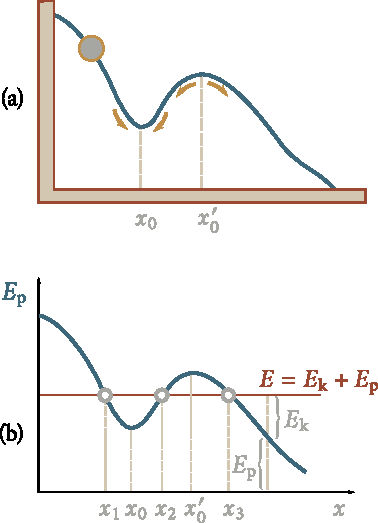
\includegraphics[scale=0.95]{figures/ch_03/fig_3_14.pdf}
			\caption[]{}
			\label{fig:3_14}
		\end{center}
	\end{minipage}
	\hspace{-0.05cm}
	\begin{minipage}[t]{0.5\linewidth}
		\begin{center}
			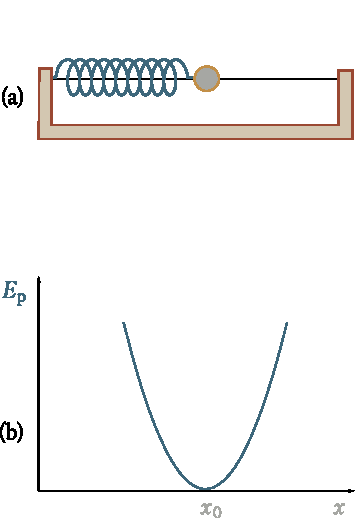
\includegraphics[scale=0.95]{figures/ch_03/fig_3_15.pdf}
			\caption[]{}
			\label{fig:3_15}
		\end{center}
	\end{minipage}
\end{figure}

Trong trường hợp biểu diễn trên \fig{3_14}, các điều kiện ~\eqref{eq:3_84} và \eqref{eq:3_85} cũng nghiệm đúng đối với $x$ bằng $x_0$ (tức là đối với cực đại của $E_{\text{p}}$). Vị trí của hòn bi xác định bằng giá trị $x$ này cũng là vị trí cân bằng . Tuy nhiên khác với sự cân bằng khi $x=x_0$ sự cân bằng này là cân bằng không bền: chỉ cần đẩy nhẹ hòn bi khỏi vị trí này, chẳng hạn như xuất hiện lực, thì lực này sẽ làm hòn bi đi ra xa vị trí $x_0$. các lực xuất hiện khi dịch chuyển hòn bi khỏi vị trí cân bằng bền (đối với vị trí $x=x_0$) có hướng sao cho chúng làm hòn bi quay về vị trí cân bằng.

Biết dạng của hàm biểu diễn thế năng, có thể đưa ra một loại các kết luận về đặc tính chuyển động của hạt. Ta hãy giải thích thêm điều này khi sử dụng đồ thị vẽ trên \fig{3_14}b. Nếu năng lượng toàn phần có giá trị được chỉ ra trên hình thì hạt có thể thực hiện chuyển động hoặc phạm vi từ $x_1$ đến  $x_2$, hoặc trong phạm vi từ  $x_3$ đến vô cùng. Trong các miền $x<x_1$ và $x_2<x<x_3$ hạt không thể lọt vào được vì thế năng sẽ không thể lớn năng lượng toàn phần (nếu điều này xảy ra thì động năng sẽ âm). Như vậy, miền $x_2<x<x_3$ là   \textbf{một hàng rào thế} mà hạt không thể xuyên qua đó khi có dự trữ đã cho của năng lượng toàn phần. Miền $x_1<x<x_2$ được gọi là  \textbf{một giếng thế }.

Nếu hạt khi chuyển động không thể ra xa vô hạn thì chuyển động được gọi là \textbf{chuyển động hữu hạn}. Nếu hạt có thể đi xa bao nhiêu tuỳ ý thì người ta gọi chuyển động là \textbf{chuyển động vô hạn}. Hạt trong giếng thế sẽ thực hiện một chuyển động hữu hạn. Chuyển động của một hạt với năng lượng toàn phần âm trong trường lực hút xuyên tâm (giả thiết rằng thế năng triệt tiêu lại vô cực) cũng là một chuyển động hữu hạn.  


\section{Định luật bảo toàn xung lượng}\label{sec:3_10}

Trong các tiết trước ta đã nghiên cứu một tích phân chuyển động cộng tính gọi là năng lượng. Ta tìm thêm một đại lượng cộng tính được bảo toàn đối với hệ kín. Với mục đích này ta hãy xét hệ $N$ hạt tương tác lẫn nhau. Giả sử ngoài các nội lực $\vec{F}_{ik}$ còn có các ngoại lực mà lực tổng hợp của chúng bằng $\vec{F}_i$ tác dụng lên hạt thứ $i$. Ta viết ~\eqn{2_10}  cho tất cả $N$ hạt:
\begin{align*}
\dot{\vec{p}}_1 &= \vec{F}_{12} + \vec{F}_{13} + \ldots + \vec{F}_{1k} + \ldots + \vec{F}_{1N} + \vec{F}_{1} = \sum_{k=2}^{N} \vec{F}_{1k} + \vec{F}_{1}\\
\dot{\vec{p}}_2 &= \vec{F}_{21} + \vec{F}_{23} + \ldots + \vec{F}_{2k} + \ldots + \vec{F}_{2N} + \vec{F}_{2} = \sum_{\substack{k=1\\(k\neq 2)}}^{N} \vec{F}_{2k} + \vec{F}_{2}\\
&\cdots \quad\quad\quad\cdots \quad\quad\quad\cdots \quad\quad\quad\cdots \quad\quad\quad\cdots\\
\dot{\vec{p}}_i &= \vec{F}_{i1} + \vec{F}_{i2} + \ldots + \vec{F}_{ik} + \ldots + \vec{F}_{iN} + \vec{F}_{i} = \sum_{\substack{k=1\\(k\neq i)}}^{N} \vec{F}_{ik} + \vec{F}_{i}\\
&\cdots \quad\quad\quad\cdots \quad\quad\quad\cdots \quad\quad\quad\cdots \quad\quad\quad\cdots\\
\dot{\vec{p}}_N &= \vec{F}_{N1} + \vec{F}_{N2} + \ldots + \vec{F}_{Nk} + \ldots + \vec{F}_{N,N-1} + \vec{F}_{N} = \sum_{k=1}^{N-1} \vec{F}_{Nk} + \vec{F}_{N}
\end{align*}

Ta hãy cộng $N$ phương trình này với nhau. Do $\vec{F}_{12}+\vec{F}_{21}=0$, v.v.vế phải chỉ còn lại các ngoại lực. Như vậy, ta đi tới hệ thức
\begin{equation}\label{eq:3_86}
\frac{\upd}{\deriv{t}}(\vec{p}_1+\vec{p}_2+\ldots+\vec{p}_N) = \vec{F}_1+\vec{F}_2+\ldots+\vec{F}_N = \sum_{i=1}^{N} \vec{F}_i
\end{equation}

Tổng các xung lượng của các hạt tạo thành hệ cơ học được gọi là \textbf{xung lượng của hệ}. Nếu ký hiệu xung lượng này là $\vec{p}$ ta có:
\begin{equation}\label{eq:3_87}
\vec{p} = \sum_{i=1}^{N} \vec{p}_i = \sum_{i=1}^{N} m_i\vec{v}_i.
\end{equation}

\noindent
từ~\eqref{eq:3_87} suy ra rằng xung lượng là một đại lượng cộng tính. 

Ta hãy viết hệ thức~\eqref{eq:3_86} dưới dạng 
\begin{equation}\label{eq:3_88}
\diff{\vec{p}}{t} = \sum_{i=1}^{N} \vec{F}_i.
\end{equation}

\noindent
Từ đó suy ra rằng khi không có các ngoại lực thì $\diffin{\vec{p}}{t}=0$. Do đó với một hệ kín $\vec{p}$ là không đổi. Điều khẳng định này là nội dung của \textbf{định luật bảo toàn xung lượng} được phát biểu như sau: \textbf{xung lượng của một hệ kín các chất điểm là không đổi}.

Ta hãy chú ý rằng xung lượng vẫn không đổi cả đối với một hệ không kín với điều kiện là các ngoại lực tổng cộng lại bằng không (xem~\eqref{eq:3_88}). Trong trường hợp khi tổng các ngoại lực không bằng không nhưng hình chiếu của tổng này lên một hướng nào đó bằng không thì thành phần của xung lượng theo phương này sẽ được bảo toàn. Thực vậy, chiếu tất cả các đại lượng của \eqn{3_88} lên một phương $x$ nào đó ta được 
\begin{equation}\label{eq:3_89}
\diff{p_x}{t} = \sum_{i=1}^{N} F_{xi}
\end{equation}

\noindent
từ đó suy ra điều khẳng định mà ta đã phát biểu. (Ta nhớ rằng $(\diffin{\vec{p}}{t})_{\text{pr. }\vec{x}}=\diffin{p_x}{t}$, xem công thức~\eqref{eq:1_40}).

Xung lượng của một hệ các hạt có thể được biểu diễn dưới dạng tích của khối lượng tổng cộng của các hạt với vận tốc của khối tâm của hệ:
\begin{equation}\label{eq:3_90}
\vec{p} = m\vec{v}_{\text{C}}
\end{equation}

\textbf{Khối tâm} (hoặc \textbf{tâm quán tính}) của hệ được định nghĩa bởi điểm C có vị trí được cho bởi bán kính vector $\vec{r}_{\text{C}}$ xác định như sau:
\begin{equation}\label{eq:3_91}
\vec{r}_{\text{C}} = \frac{m_1\vec{r}_1+m_2\vec{r}_2+\ldots+m_N\vec{r}_N}{m_1+m_2+\ldots+m_N} = \frac{\sum_{i=1}^N m_i\vec{r}_i}{\sum_{i=1}^N m_i} = \frac{1}{m} \sum_{i=1}^N m_i\vec{r}_i
\end{equation}

\noindent
Ở đây $m_i$  là khối lượng của hạt thứ $i$, $\vec{r}_i$ là bán kính của vector xác định vị trí của hạt này, $m$ là khối lượng của hệ.

Các tọa độ Decartes của khối tâm bằng các hình chiếu của $\vec{r}_{\text{C}}$ lên các trục tọa độ:
\begin{equation}\label{eq:3_92}
x_{\text{C}} = \frac{1}{m} \sum_{i=1}^N m_i x_i,\quad y_{\text{C}} = \frac{1}{m} \sum_{i=1}^N m_i y_i,\quad
z_{\text{C}} = \frac{1}{m} \sum_{i=1}^N m_i z_i.
\end{equation}

\noindent
Chú ý rằng trong một trọng trường đều, khối tâm trùng với trọng tâm của hệ.

Vận tốc của khối tâm có được bằng cách lấy đọa hàm bán kính vector~\eqref{eq:3_91} theo thời gian:
\begin{equation*}
\vec{v}_{\text{C}} = \dot{\vec{r}}_{\text{C}} = \frac{1}{m}\sum_{i=1}^N m_i\dot{\vec{r}}_i = \frac{1}{m} \sum_{i=1}^N m_i\vec{v}_i = \frac{\vec{p}}{m}
\end{equation*}

\noindent
(xem~\eqref{eq:3_87}). Từ đây suy ra công thức~\eqref{eq:3_90}.

Đối với hệ kín thì $\vec{p}=m\vec{v}_{\text{C}}=\text{constant}$. Do đó, khối tâm của một hệ kín hoặc chuyển động thằng và đều hoặc đứng yên.

Hệ quy chiếu trong đó khối tâm đừng nghỉ được gọi là \textbf{hệ khối tâm} hoặc \textbf{hệ k.t}. Hệ này rõ ràng là một hệ quán tính.

Hệ quy chiếu gắn với các máy đo được gọi là \textbf{hệ phòng thí nghiệm} hoặc \textbf{hệ p}.

\section{Sự va chạm của hai vật}\label{sec:3_11}

Khi các vật va chạm với nhau chúng bị biến dạng. Khi đó, động năng mà các vật đã có trước lúc va chạm chuyển một phần hoặc toàn bộ thành thế năng biến dạng đàn hồi và thành nội năng của các vật. Sự tăng nội năng của các vật được kèm theo sự tăng nhiệt độ của chúng.

Có hai dạng va chạm giới hạn: va chạm tuyệt đối đàn hồi và tuyệt đối không đàn hồi. Va chạm được gọi là \textbf{tuyệt đối đàn hồi} nếu khi va chạm cơ năng của các vật không chuyển thành các dạng năng lượng, không cơ học khác. Trong va chạm đó động năng chuyển hoàn toàn hoặc một phần thành thế năng biến dạng đàn hồi. Sau đó các vật trở lại hình dạng ban đầu và đẩy nhau. Kết quả là thế năng biến dạng đàn hồi lại chuyển thành động năng và các vật bay ra với các vận tốc có độ lớn và hướng được xác định bằng hai điều kiện, đó là sự bảo toàn năng lượng toàn phần và bảo toàn xung lượng toàn phần của hệ vật.

Sự va chạm tuyệt đối không đàn hồi được đặc trưng ở chỗ là thế năng biến dạng không xuất hiện: động năng của các vật hoàn toàn hoặc một phần biến thành nội năng; sau va chạm các vật bị va chạm hoặc chuyển động với cùng một vận tốc hoặc đứng nghỉ. Trong sự va chạm tuyệt đối không đàn hồi chỉ có định luật bảo toàn cơ năng không được tuân theo, nghĩa là xảy ra định luật bảo toàn năng lượng tổng cộng thuộc các dạng khác nhau là cơ năng và nội năng. 

Trước hết ta hãy nghiên cứu sự va chạm tuyết đối không đàn hồi của hai hạt  (chất điểm) tạo thành một hệ kín. Giả thử các khối lượng của các hạt bằng $m_1$ và $m_2$, còn các vận tốc trước lúc va chạm là $\vec{v}_{10}$và $\vec{v}_{20}$. Theo định luật bảo toàn, xung lượng tổng cộng của các hạt sau va chạm cũng phải như trước lúc va chạm:
\begin{equation}\label{eq:3_93}
m_1\vec{v}_{10} + m_2\vec{v}_{20} = m_1\vec{v} + m_2\vec{v} = (m_1+m_2) \vec{v}
\end{equation}

\noindent
($\vec{v}$ là vận tốc chung cho cả hai hạt sau va chạm). Từ \eqref{eq:3_93} suy ra
\begin{equation}\label{eq:3_94}
\vec{v} = \frac{m_1\vec{v}_{10} + m_2\vec{v}_{20}}{m_1+m_2}.
\end{equation}

\noindent
Đối với các tính toán thực hành cần phải chiếu hệ thức \eqref{eq:3_94} lên các phương được chọn một cách thích hợp.


Bây giờ ta nghiên cứu sự va chạm tuyệt đối đàn hồi. Hơn nữa hạn chế ở trường hợp va chạm xuyên tâm của hai quả cầu đồng tính. Va chạm được gọi là va chạm xuyên tâm nếu các quả cầu trước lúc va chạm chuyển động dọc theo đường thẳng đi qua các tâm của chúng. Trong va chạm xuyên tâm sự va chạm có thể xảy ra nếu:  (1) các quả cầu chuyển động đến gặp nhau  (\fig{3_16}a), và (2) một quả cầu đuổi theo quả cầu kia (\fig{3_16}b).

\begin{figure}[!htb]
	\begin{center}
		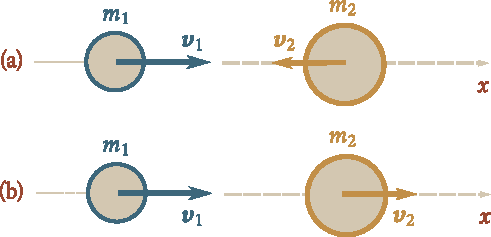
\includegraphics[scale=1]{figures/ch_03/fig_3_16.pdf}
		\caption[]{}
		\label{fig:3_16}
	\end{center}
\end{figure}

Ta sẽ giả thiết rằng các quả cầu tạo thành một hệ kín hoặc các ngoại lực đặt lên các quả cầu đều cân bằng với nhau. Ngoài ra, ta sẽ coi rằng các quả cầu không quay.

Ta ký hiệu các khối lượng của các quả cầu là $m_1$ và $m_2$, các vận tốc của các quả cầu trước lúc va chạm là $\vec{v}_{10}$ và $\vec{v}_{20}$ và cuối cùng các vận tốc sau va chạm là $\vec{v}_{1}$ và $\vec{v}_{2}$. Ta hãy viết các phương trình bảo toàn năng lượng và xung lượng:
\begin{align}
\frac{m_1\vec{v}_{10}^2}{2} + \frac{m_2\vec{v}_{20}^2}{2} &= \frac{m_1\vec{v}_{1}^2}{2} + \frac{m_2\vec{v}_{2}^2}{2}\label{eq:3_95}\\
m_1\vec{v}_{10} + m_2\vec{v}_{20} &= m_1\vec{v}_{1} + m_2\vec{v}_{2}.\label{eq:3_96}
\end{align}

\noindent
Để ý rằng  $(\vec{a}_2-\vec{b}_2)=(\vec{a}-\vec{b})(\vec{a}+\vec{b})$, ta đưa \eqn{3_95} về dạng
\begin{equation}\label{eq:3_97}
m_1(\vec{v}_{10}-\vec{v}_{1})(\vec{v}_{10}+\vec{v}_{1}) = m_2(\vec{v}_{2}-\vec{v}_{20})(\vec{v}_{2}+\vec{v}_{20}).
\end{equation}

\noindent
Ta biến đổi hệ thức \eqref{eq:3_96} như sau:
\begin{equation}\label{eq:3_98}
m_1(\vec{v}_{10}-\vec{v}_{1}) = m_2(\vec{v}_{2}-\vec{v}_{20}).
\end{equation}

Vì lý do đối xứng có thể khẳng định rằng các vận tốc của các quả cầu sau va chạm sẽ hướng theo cùng một đường thẳng mà trước va chạm các tâm của các quả cầu chuyển động dọc theo đó. Do đó mọi vector trong ~\eqref{eq:3_97} và \eqref{eq:3_98} đều là đồng phương. Đối với các vector đồng phương  $\vec{a}, \vec{b}, \vec{c}$, từ $\vecdot{a}{b}=\vecdot{a}{c}$ suy ra $\vec{b}=\vec{c}$. Do đó, so sánh ~\eqref{eq:3_97} và \eqref{eq:3_98} có thể kết luận rằng
\begin{equation}\label{eq:3_99}
\vec{v}_{10} + \vec{v}_{1} = \vec{v}_{2} + \vec{v}_{20}.
\end{equation}

\noindent
Nhân \eqref{eq:3_99} với $m_2$ và lấy \eqref{eq:3_98} trừ đi kết quả nhận được, và sau đó nhân \eqref{eq:3_99} với $m_1$ và cộng kết quả với  \eqref{eq:3_98}, ta thu được các vận tốc của các quả cầu sau va chạm:
\begin{equation}\label{eq:3_100}
\vec{v}_1 = \frac{2m_2\vec{v}_{20}+(m_1-m_2)\vec{v}_{10}}{m_1+m_2},\quad \vec{v}_2 = \frac{2m_1\vec{v}_{10}+(m_2-m_1)\vec{v}_{20}}{m_1+m_2}.
\end{equation}

\noindent
Đối với các phép tính bằng số cần phải chiếu hệ thức ~\eqref{eq:3_100} lên trục $x$ mà dọc theo đó các quả cầu chuyển động (xem \fig{3_16}).

Ta chú ý rằng các vận tốc của các quả cầu sau va chạm tuyệt đối đàn hồi không thể giống nhau. Thực vậy, làm cân bằng với nhau các biểu thức ~\eqref{eq:3_100} đối với $\vec{v}_1$ và $\vec{v}_2$ và thực hiện các phép biến đổi ta được 
\begin{equation*}
\vec{v}_{10} = \vec{v}_{20}.
\end{equation*}

\noindent
Do đó, muốn cho các vận tốc của các quả cầu sau va chạm là như nhau, thì chúng phải có các vận tốc như nhau trước lúc va chạm, nhưng trong trường hợp này sự va chạm không thể xảy ra. Từ đây suy ra rằng điều kiện bằng nhau của các vận tốc của các quả cầu sau khi va chạm sẽ trái ngược với định luật bảo toàn năng lượng. Như vậy trong va chạm không đàn hồi cơ năng không được bảo toàn - nó chuyển một phần thành nội năng của các vật bị va chạm để làm nóng chúng. 

Ta hãy xét trường hợp khi các khối lượng của các quả cầu va chạm nhau bằng: $m_1=m_2$. Từ ~\eqref{eq:3_100} suy ra rằng với điều kiện này 
\begin{equation*}
\vec{v}_{1} = \vec{v}_{20}\quad \vec{v}_{2} = \vec{v}_{10}
\end{equation*}

\noindent
nghĩa là khi va chạm các quả cầu trao đổi các vận tốc cho nhau. Đặc biệt, nếu một trong các quả cầu có khối lượng giống nhau, chẳng hạn quả cầu thứ hai, trước khi va chạm đứng yên, thì sau va chạm nó chuyển động với vận tốc như vận tốc ban đầu của quả cầu thứ nhất, còn quả cầu thứ nhất sau va chạm sẽ lại đứng yên. 

Nhờ các công thức~\eqref{eq:3_100} có thể xác định vận tốc của quả cầu sau va chạm đàn hồi vào một thành đứng yên hoặc chuyển động   (có thể coi nó như một quả cầu có khối lượng $m_2$ lớn vô cùng và có bán kính lớn vô cùng). Chia tử số và mẫu số của các biểu thức ~\eqref{eq:3_100} cho $m_2$ và bỏ qua các số hạng chứa thừa số $m_1/m_2$, ta có
\begin{equation*}
\vec{v}_{1} = 2\vec{v}_{20}-\vec{v}_{10}\quad \vec{v}_{2} = \vec{v}_{20}.
\end{equation*}

\noindent
Kết quả cho ta thấy vận tốc của thành là không đổi . Vận tốc của quả cầu, nếu thành đứng yên ($\vec{v}_{20}=0$), sẽ biến đổi theo chiều ngược lại; trong trường hợp thành chuyển động trị số của vận tốc của quả cầu cũng biến đổi  (tăng lên $2v_{20}$ nếu thành chyển động đến gặp quả cầu, và giảm đi $2v_{20}$, nếu thành 'đi' cùng chiều và quả cầu đuối theo nó).

\begin{figure}[!htb]
	\begin{center}
		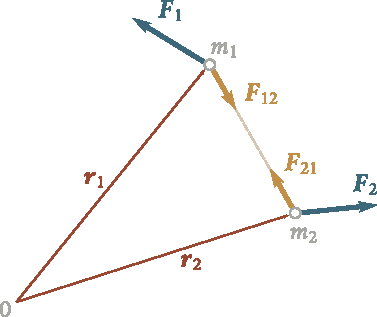
\includegraphics[scale=1]{figures/ch_03/fig_3_17.pdf}
		\caption[]{}
		\label{fig:3_17}
	\end{center}
\end{figure}

\section{Định luật bảo toàn momen xung lượng}\label{sec:3_12}
   
Ta đã biết hai đại lượng cộng tính được bảo toàn: năng lượng và xung lượng. Bây giờ ta tìm một đại lượng thứ ba như thế. Muốn vậy, ta xét một hệ gồm hai hạt tương tác lẫn nhau chịu tác dụng của các ngoại lực (\fig{3_17}). Các phương trình chuyển động của các hạt có dạng:
\begin{equation*}
m_1\dot{\vec{v}}_1 = \vec{F}_{12} + \vec{F}_1,\quad m_2\dot{\vec{v}}_2 = \vec{F}_{21} + \vec{F}_2.
\end{equation*}

\noindent
Ta nhân vector bên trái phương trình thứ nhất với bán kính vector $\vec{r}_1$ của hạt thứ nhất, còn phương trình thứ hai với bán kính vector $\vec{r}_2$ của hạt thứ hai:
\begin{equation}\label{eq:3_101}
\begin{cases}
& \!\!\!\! m_1(\vec{r}_1\times\dot{\vec{v}}_1) = \vecprodind{r}{1}{F}{12} + \vecprodind{r}{1}{F}{1}\\
& \!\!\!\! m_2(\vec{r}_2\times\dot{\vec{v}}_2) = \vecprodind{r}{2}{F}{21} + \vecprodind{r}{2}{F}{2}.
\end{cases}
\end{equation}

Tích vector có dạng $\vec{r}\times\dot{\vec{v}}$ tương đương với biểu thức $\diffin{(\vec{r}\times\dot{\vec{v}})}{t}$. Thực vậy, theo \eqn{1_55}
\begin{equation}\label{eq:3_102}
\frac{\upd}{\deriv{t}}(\vec{r}\times\dot{\vec{v}}) = \vec{r}\times\dot{\vec{v}} + \dot{\vec{r}}\times\vec{v} = \vec{r}\times\dot{\vec{v}}
\end{equation}

\noindent
vì $\dot{\vec{r}}\times\vec{v}=\vec{v}\times\vec{v}=0$. Nếu thay vào các công thức~\eqref{eq:3_101} và chú ý rằng $\vec{F}_{21}=-\vec{F}_{12}$, ta đi tới các phương trình
\begin{equation}\label{eq:3_103}
\begin{cases}
& \!\!\!\! m_1\,\dfrac{\upd}{\deriv{t}}(\vec{r}_1\times\vec{v}_1) = \vecprodind{r}{1}{F}{12} + \vecprodind{r}{1}{F}{1}\\[10pt]
& \!\!\!\! m_2\,\dfrac{\upd}{\deriv{t}}(\vec{r}_2\times\vec{v}_2) = - \vecprodind{r}{2}{F}{12} + \vecprodind{r}{2}{F}{2}.
\end{cases}
\end{equation}

Khối lượng là một đại lượng vô hướng không đổi. Do đó có thể đưa nó vào dưới dấu đạo hàm theo thời gian và vào tích vector: 
\begin{equation*}
m\,\frac{\upd}{\deriv{t}}(\vec{r}\times\vec{v}) = \frac{\upd}{\deriv{t}}(\vec{r}\times m\vec{v}) = \frac{\upd}{\deriv{t}}(\vec{r}\times\vec{p}).
\end{equation*}

\noindent
Chú ý tới điều này ta cộng các phương trình~\eqref{eq:3_103} với nhau. Kết quả ta được: \begin{equation*}
\frac{\upd}{\deriv{t}}(\vecprodind{r}{1}{p}{1} + \vecprodind{r}{2}{p}{2}) = (\vec{r}_1-\vec{r}_2)\times\vec{F}_{12} + \vecprodind{r}{1}{F}{1} + \vecprodind{r}{2}{F}{2}.
\end{equation*}

\noindent
Các vector $\vec{r}_1-\vec{r}_2$ và $\vec{F}_{12}$ là đồng phương; do đó tích vector của chúng bằng không. Như vậy ta đi tới hệ thức:
\begin{equation}\label{eq:3_104}
\frac{\upd}{\deriv{t}}(\vecprodind{r}{1}{p}{1} + \vecprodind{r}{2}{p}{2}) = \vecprodind{r}{1}{F}{1} + \vecprodind{r}{2}{F}{2}.
\end{equation}

\noindent
Nếu hệ là kín thì vế phải của hệ thức này bằng không và do đó 
\begin{equation*}
\vecprodind{r}{1}{p}{1} + \vecprodind{r}{2}{p}{2} = \text{constant}.
\end{equation*}

\noindent
Ta đã đi tới một đại lượng cộng tính được bảo toàn mà người ta gọi là momen xung lượng\footnote{Tên gọi cũ của đại lượng này là momen động lượng} đối với điểm $O$ (xem \fig{3_17}).

Đối với một lấy riêng lẻ thì giả vector
\begin{equation}\label{eq:3_105}
\vec{L} = \vecprod{r}{p} = \vec{r}\times m\vec{v}.
\end{equation}

\noindent
được gọi là \textbf{momen xung lượng đối với điểm $O$}.

Momen xung lượng của hệ đối với điểm $O$ là tổng vector các momen xung lượng của các hạt tham gia vào hệ:
\begin{equation}\label{eq:3_106}
\vec{L} = \sum_{i}\vec{L}_i = \sum_{i} \vecprodind{r}{i}{p}{i}.
\end{equation}

Hình chiều của vector~\eqref{eq:3_105} trên một trục $z$ nào đó được gọi là \textbf{momen xung lượng của hạt đối với trục này}:
\begin{equation}\label{eq:3_107}
L_z = (\vecprod{r}{p})_{\text{pr.},\vec{z}}.
\end{equation}

\noindent
Một cách tương tự, \textbf{momen xung lượng của hệ đối với trục $z$} được định nghĩa là đại lượng vô hướng 
\begin{equation}\label{eq:3_108}
L_z = \sum_i (\vecprodind{r}{i}{p}{i})_{\text{pr.},\vec{z}}.
\end{equation}

%\begin{figure}[t]
%	\begin{center}
%		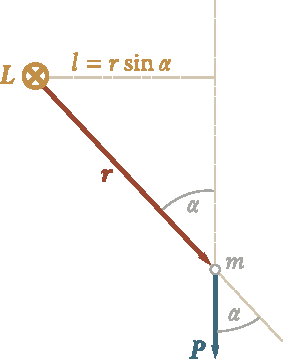
\includegraphics[scale=1]{figures/ch_03/fig_3_18.pdf}
%		\caption[]{}
%		\label{fig:3_18}
%	\end{center}
%	%	\vspace{-0.7cm}
%\end{figure}

\noindent
Từ \fig{3_18} rõ ràng là module của vector momen xung lượng của hạt bằng:
\begin{equation}\label{eq:3_109}
L = rp\sin\alpha = lp
\end{equation}

\noindent
trong đó $l=r\sin\alpha$ là độ dài của đường vuông góc hạ từ điểm $O$ lên đường thẳng mà xung lượng của hạt hướng dọc theo nó. Độ dài này được gọi là \textbf{tay đòn của xung lượng đối với điểm $O$}. Hình~\ref{fig:3_18} được thực hiện với giả thiết là điểm $O$ mà ta tính momen đối với nó là vector $\vec{p}$ đều nằm trong mặt phẳng hình vẽ. Vector $\vec{L}$ vuông góc với mặt phẳn hình vẽ và hướng ra xa chúng ta.

Ta hãy xét hai ví dụ tiêu biểu. 
\begin{enumerate}[1.]
	\item Giả sử hạt chuyển động dọc theo đường thẳng vẽ trên \fig{3_18} bằng đường chấm chấm. Trong trường hợp này momen xung lượng của hạt có thể biến đổi chỉ về độ lớn. Module của momen bằng:
	\begin{equation}\label{eq:3_110}
	L = mvl
	\end{equation}

	\noindent
	hơn nữa tay đòn $l$ không biến đổi.
	\item Hạt có khối lượng $m$ chuyển động theo đường tròn bán kính $R$  (\fig{3_19}). Momen xung lượng của hạt đối với tâm $O$ của đường tròn về module bằng 
	\begin{equation}\label{eq:3_111}
	L = mvR
	\end{equation}

	\noindent
	Vector $\vec{L}$ vuông góc với mặt phẳng của đường tròn, trong khi dọc hướng chuyển động cả hạt và vector $\vec{L}$ tạo thành hệ đinh ốc thuận. Vì tay đòn bằng $R$ là không đổi nên momen xung lượng có thể chỉ biến đổi do sự biến đổi module của vận tốc. Khi hạt chuyển động tròn đều momen xung lượng không đổi cả về độ lớn lẫn hướng.
\end{enumerate}

\begin{figure}[!htb]
	\begin{minipage}[t]{0.5\linewidth}
		\begin{center}
			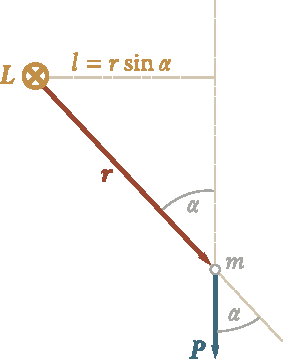
\includegraphics[scale=0.95]{figures/ch_03/fig_3_18.pdf}
			\caption[]{}
			\label{fig:3_18}
		\end{center}
	\end{minipage}
	\hspace{-0.05cm}
	\begin{minipage}[t]{0.5\linewidth}
		\begin{center}
			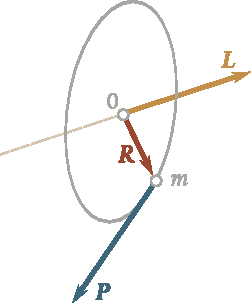
\includegraphics[scale=0.95]{figures/ch_03/fig_3_19.pdf}
			\caption[]{}
			\label{fig:3_19}
		\end{center}
	\end{minipage}
\end{figure}

Giả vector
\begin{equation}\label{eq:3_112}
\vec{M} = \vecprod{r}{F}
\end{equation}

\noindent
được gọi là \textbf{moment của lực $\vec{F}$ đối với điểm O}, mà tại đó ta vẽ bán kính vector $\vec{r}$ của điểm đặt của lực (\fig{3_20}). Từ hình vẽ rõ rằng là có thể biểu diễn module của moment lực dưới dạng 
\begin{equation}\label{eq:3_113}
M = rF\sin\alpha = lF
\end{equation}

\noindent
trong đó $l=r\sin\alpha$ là \textbf{tay đòn của lực đối với điểm O} (tức là độ dài của đường vuông góc hạ từ điểm $O$ lên đường thẳng dọc theo đó lực tác dụng) 

Hình chiếu của vector $\vec{M}$ lên một trục $z$ nào đó đi qua điểm $O$ mà $\vec{M}$ được xác định được gọi là \textbf{moment của lực đối với trục} này: 
\begin{equation}\label{eq:3_114}
M_z = \vecprod{r}{F}_{\text{pr.},\vec{z}}.
\end{equation}

\begin{figure}[!htb]
	\begin{minipage}[t]{0.5\linewidth}
		\begin{center}
			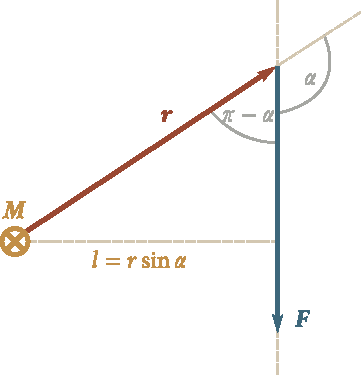
\includegraphics[scale=0.9]{figures/ch_03/fig_3_20.pdf}
			\caption[]{}
			\label{fig:3_20}
		\end{center}
	\end{minipage}
	\hspace{-0.05cm}
	\begin{minipage}[t]{0.5\linewidth}
		\begin{center}
			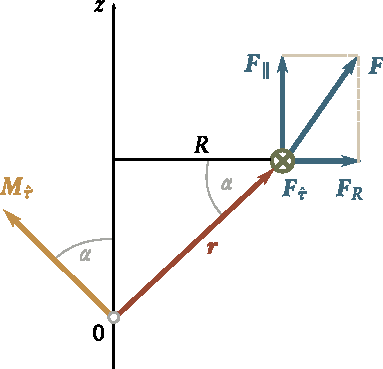
\includegraphics[scale=0.9]{figures/ch_03/fig_3_21.pdf}
			\caption[]{}
			\label{fig:3_21}
		\end{center}
	\end{minipage}
\end{figure}

\noindent
Ta phân tích vector lực $\vec{F}$ (\fig{3_21}) thành ba thành phần vuông góc với nhau: $\vec{F}_{\parallel}$ là thành phần song song với trục $z$, $\vec{F}_R$ là thành phần vuông góc với trục $z$ và tác dụng dọc theo đường thằng đi qua trục, và cuối cùng,  $\vec{F}_{\hatvec{\tau}}$ là thành phần vuông góc với mặt phẳng đi qua trục và điểm đặt của lực (thành phần này được ký hiệu trên hình vẽ bằng một vòng tròn nhỏ có dấu chữ thập). Nếu tưởng tượng một đường tròn bán kính $R$ với tâm trên trục $z$ thì thành phần $\vec{F}_{\hatvec{\tau}}$ sẽ hướng theo tiếp tuyến của đường tròn này. Moment của lực $\vec{F}$ đối với điểm $0$ bằng tổng các momen của các thành phần: $\vec{M}=\vec{M}_{\parallel}+\vec{M}_R+\vec{M}_{\hatvec{\tau}}$. Các vector $\vec{M}_{\parallel}$, và $\vec{M}_R$ đều vuông góc với trục $z$, do đó hình chiếu của chúng trên trục $z$ bằng không. Momen $\vec{M}_{\hatvec{\tau}}$ có module bằng $rF_{\hatvec{\tau}}$ và tạo với trục $z$ một góc $\alpha$ có cosine bằng $R/r$. Do đó moment của các thành phần $\vec{F}_{\hatvec{\tau}}$ đối với trục $z$ có độ lớn $\vec{M}_{\hatvec{\tau}}\cos\alpha=RF_{\hatvec{\tau}}$. Như vậy, moment của lực $\vec{F}$ đối với trục $z$ bằng:
\begin{equation}\label{eq:3_115}
M_z = RF_{\hatvec{\tau}}.
\end{equation}

\noindent
Cho đến nay ta đã hiểu $F_{\hatvec{\tau}}$ là module của thành phần $\vec{F}_{\hatvec{\tau}}$. Tuy vậy có thể coi $F_{\hatvec{\tau}}$ như hình chiếu của vector $\vec{F}$ lên vector đơn vị $\hatvec{\tau}$, tiếp tuyến của đường tròn bán kính $R$ và hướng sao cho sự chuyển động trên đường tròn theo hướng $\hatvec{\tau}$ tạo với hướng của trục $z$ một hệ đinh ốc thuận. Với cách giải thích như thế về  $F_{\hatvec{\tau}}$, \eqn{3_115} sẽ xác định cả dấu $M_z$.

Momen của lực $\vec{M}$ đặc trưng cho khả năng của lực làm quay vật quanh điểm mà momen được lấy đối với nó. Ta hãy chú ý rằng trong trường hợp khi vật có thể quay đối với điểm $O$ một cách tùy ý, thì dưới tác dụng của lực vật quay xung quanh trục vuông góc với mặt phẳng chứa lực và điểm $O$, nghĩa là xung quanh trục trùng với hướng của moment của lực đối với điểm này.

Moment của lực đối với trục $z$ này đặc trưng khả năng của lực làm quay vật xung quanh trục này. Các thành phần $\vec{F}_{\parallel}$ và $\vec{F}_{R}$ không thể gây ra sự quay xung qianh trục $z$. Sự quay đó chỉ có thể gây ra bởi thành phần $\vec{F}_{\hatvec{\tau}}$, hơn nữa thành phần này thực hiện sự quay càng có kết quả khi tay đòn $R$ của nó càng lớn. 

Hai lực ngược chiều, cùng phương và có độ lớn bằng nhau được gọi là một \textbf{ngẫu lực} (\fig{3_22}). Khoảng cách $l$ giữa các đường thẳng dọc theo đó các lực tác dụng được  gọi là \textbf{tay đòn của ngẫu lực}. Moment tổng của các lực $\vec{F}_1$ và $\vec{F}_2$ tạo thành ngẫu lực bằng
\begin{equation*}
\vec{M} = \vecprodind{r}{1}{F}{1} + \vecprodind{r}{2}{F}{2}.
\end{equation*}

\noindent
Nếu để ý tới $\vec{F}_1=-\vec{F}_2$, thì có thể viết: 
\begin{equation}\label{eq:3_116}
\vec{M} = -\vecprodind{r}{1}{F}{2} + \vecprodind{r}{2}{F}{2} = (\vec{r}_2 - \vec{r}_1)\times\vec{F}_2 = \vecprodind{r}{12}{F}{2}
\end{equation}

\noindent
trong đó $\vec{r}_{12}=\vec{r}_2-\vec{r}_1$ là vector vẽ từ điểm đặt của lực $\vec{F}_1$ tới điểm đặt của lực $\vec{F}_2$. Biểu thức~\eqref{eq:3_116} không phụ thuộc vào việc chọn điểm $O$. Do đó moment ngẫu lực đối với mọi điển là như nhau. Vector moment ngẫu lực vuông góc với mặt phẳng chứa các lực (xem \fig{3_22})  và về trị số bằng tích của module của một trong các lực với cánh tay đòn. 

\begin{figure}[!htb]
	\begin{minipage}[t]{0.5\linewidth}
		\begin{center}
			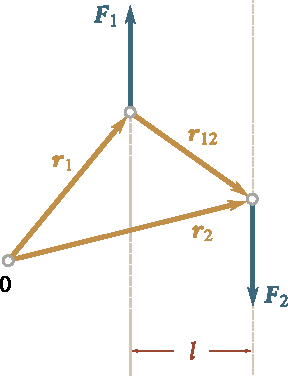
\includegraphics[scale=0.95]{figures/ch_03/fig_3_22.pdf}
			\caption[]{}
			\label{fig:3_22}
		\end{center}
	\end{minipage}
	\hspace{-0.05cm}
	\begin{minipage}[t]{0.5\linewidth}
		\begin{center}
			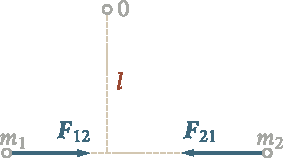
\includegraphics[scale=0.95]{figures/ch_03/fig_3_23.pdf}
			\caption[]{}
			\label{fig:3_23}
		\end{center}
	\end{minipage}
\end{figure}

Các lực tương tác giữa các hạt tác dụng về các phía ngược nhau dọc theo cùng một đường thẳng (\fig{3_23}). Các module của chúng đối với điểm $O$ tùy ý đều bằng nhau về độ lớn và ngược nhau về hướng. Do đó các moment của các nội lực cân bằng nhau từng đôi một, và tổng các moment của tất cả các nội lực đối với một hệ hạt bất kỳ, cụ thể là đối với một vật rắn, sẽ luôn bằng không: 
\begin{equation}\label{eq:3_117}
\sum\vec{M}_{\text{int}} = 0.
\end{equation}

Theo các phương trình~\eqref{eq:3_106} và~\eqref{eq:3_112}, có thể viết \eqref{eq:3_104} như sau:
\begin{equation}\label{eq:3_118}
\frac{\upd}{\deriv{t}}\vec{L} = \sum\vec{M}_{\text{ext}}.
\end{equation}

\noindent
Công thức này giống công thức~\eqref{eq:3_88}. Từ sự so sánh các công thức này suy ra rằng, tương tự như đạo hàm theo thời gian của xung lượng của hệ bằng tổng các ngoại lực, đạo hàm theo thời gian của momen xung lượng bằng tổng moment của các ngoại lực. 

Từ~\eqn{3_118} suy ra rằng khi không có các ngoại lực thì $\diffin{\vec{L}}{t}$. Do đó đói với một hệ kín $\vec{L}$ là không đổi. Sự khẳng định này là nội dung của định luật bảo toàn momen xung lượng được diễn đạt như sau: \textbf{momen xung lượng của một hệ kín các chất đểm là không đổi}.

Ta đã chứng minh hệ thức~\eqref{eq:3_118} đối với hệ gồm hai hạt. Tuy vậy dễ dàng khái quát hóa cho trường hợp đối với một số hạt bất kỳ. Ta hãy viết phương trình chuyển động của các hạt:
\begin{align*}
m_1\dot{\vec{v}}_1 &= \sum_k \vec{F}_{1k} + \vec{F}_1\\
\cdots & \quad\cdots \quad\cdots\\
m_i\dot{\vec{v}}_i &= \sum_k \vec{F}_{ik} + \vec{F}_i\\
\cdots & \quad\cdots \quad\cdots\\
m_N\dot{\vec{v}}_N &= \sum_k \vec{F}_{Nk} + \vec{F}_N
\end{align*}

\noindent
Nhân mỗi phương trình với bán kính vector tương ứng ta được (xem~\eqref{eq:3_102}):
\begin{align*}
\frac{\upd}{\deriv{t}}(\vecprodind{r}{1}{p}{1}) &= \sum_k \vecprodind{r}{1}{F}{1k} + \vecprodind{r}{1}{F}{1}\\
\cdots\quad\quad\cdots & \quad\quad\cdots \quad\quad\cdots \quad\quad\cdots\\
\frac{\upd}{\deriv{t}}(\vecprodind{r}{i}{p}{i}) &= \sum_k \vecprodind{r}{i}{F}{ik} + \vecprodind{r}{i}{F}{i}\\
\cdots\quad\quad\cdots & \quad\quad\cdots \quad\quad\cdots \quad\quad\cdots\\
\frac{\upd}{\deriv{t}}(\vecprodind{r}{N}{p}{N}) &= \sum_k \vecprodind{r}{N}{F}{Nk} + \vecprodind{r}{N}{F}{N}.
\end{align*}

\noindent
Ta hãy cộng tất cả $N$ phương trình với nhau:
\begin{equation*}
\frac{\upd}{\deriv{t}} \sum_i \vec{L}_i = \sum_{\substack{i=k\\(i\neq k)}} \vecprodind{r}{i}{F}{ik} + \vecprodind{r}{i}{F}{i}.
\end{equation*}

\noindent
Tổng thứ nhất ở vế phải là tổng các moment của tất cả các nội lực, như ta đã chứng tỏ, là bằng không (xem~\eqref{eq:3_117}). Tổng thứ hai ở vế phải là tổng các moment của các ngoại lực. Do đó ta đi tới công thức~\eqref{eq:3_118}.

Ta chú ý rằng momen xung lượng là đổi cả đối với hệ không kín với điểu kiện momen tổng của các ngoại lực bằng không  (xem~\eqref{eq:3_118}).

Chiếu tất cả các đại lượng tham gia vào  \eqn{3_118} lên một phương $z$ nào đó, ta được hệ thức:
\begin{equation}\label{eq:3_119}
\frac{\upd}{\deriv{t}} L_z = \sum M_{z,\text{ext}}
\end{equation}

\noindent
theo hệ thức này đọa hàm theo thời gian của momen xung lượng của hệ đối với trục $z$ là bằng tổng các moment của ngoại lực đối với trục này. 

Từ~\eqn{3_119} suy ra rằng trong trường hợp khi tổng các moment của các ngoại lực đối với một trục nào đó bằng không, thì momen xung lượng của hệ đối với trục này là không đổi.

\section{Chuyển động trong trường lực xuyên tâm }\label{sec:3_13}

Ta hãy nghiên cứu một hạt nằm trong trường lực xuyên tâm. Ta hãy nhớ lại hướng của lực tác dụng lên hạt tại một điểm bất kỳ của trường đó đi qua điểm $O$-tâm của trường, còn độ lớn của lực chỉ phụ thuộc vào khoảng cách đến tâm này. Dễ dàng hiểu được rằng sự phụ thuộc của lực $\vec{F}$ vào $\vec{r}$ có dạng;
\begin{equation}\label{eq:3_120}
\vec{F} = f(r) \vecuni{r}
\end{equation}

\noindent
trong đó $\vecuni{r}$ là chuẩn của bán kính vector (\fig{3_24}), còn $f(r)$ là hình chiếu của vector lực lên phương của bán kính vector, tức là $F_r$. Đối với lực đẩy; hàm $f(r)$ là dương; đối với lực hút; hàm $f(r)$ là âm. Hình ~\ref{fig:3_24} vẽ cho trường hợp đẩy hạt khối tâm lực. Công thức ~\eqref{eq:3_120} dĩ nhiên chỉ đúng trong trường hợp nếu gốc toạ độ (nghĩa là điểm mà bán kính vector được vẽ từ đó) đặt vào tâm của trường. 

\begin{figure}[!htb]
	\hspace{-0.5cm}
	\begin{minipage}[t]{0.5\linewidth}
		\begin{center}
			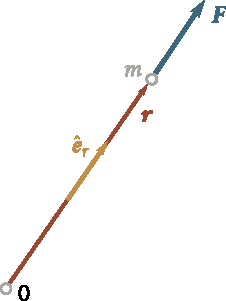
\includegraphics[scale=0.9]{figures/ch_03/fig_3_24.pdf}
			\caption[]{}
			\label{fig:3_24}
		\end{center}
	\end{minipage}
	\hspace{-0.5cm}
	\begin{minipage}[t]{0.5\linewidth}
		\begin{center}
			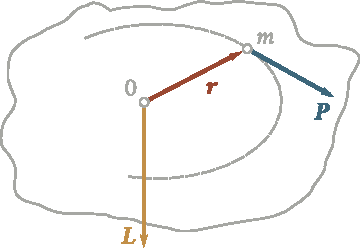
\includegraphics[scale=0.95]{figures/ch_03/fig_3_25.pdf}
			\caption[]{}
			\label{fig:3_25}
		\end{center}
	\end{minipage}
\end{figure}

Moment của lực ~\eqref{eq:3_120} đối với điểm $O$ rõ ràng là bằng không. Điều này suy ra từ chỗ tay đòn của lực  là bằng không. Từ đây, theo \eqn{3_118} suy ra rằng momen xung lượng của hạt chuyển động trong trường lực xuyên tâm là không đổi. Vector $\vec{L}=\vecprod{r}{p}$ tại mỗi thời điểm đều vuông góc với mặt phẳng tạo bởi các vector $\vec{r}$ và $\vec{p}$ (\fig{3_25}). Nếu  $\vec{L}=\text{constant}$, thì mặt phẳng này sẽ cố định. Như vậy, khi hạt chuyển động trong trường lực xuyên tâm, bán kính vector của nó luôn luôn nằm trong một mặt phẳng. Vector $\vec{p}$ cũng luôn luôn nằm trong chính mặt phẳng này. Do đó quỹ đạo của hạt là một đường cong phẳng. Mặt phẳng chứa quỹ đạo đi qua tâm của trường (xem \fig{3_25}).

Trên hình~\ref{fig:3_26} ta vẽ một đoạn quỹ đạo của hạt ( vector $\vec{L}$ được hướng ra sau hình vẽ). Trong thời gian $\deriv{t}$ bán kính vector của hạt vạch nên diện tích gạch gạch $\deriv{S}$. Diện tích này bằng một nửa diện tích hình bình hành được tạo bởi các vector $\vec{r}$ và $\vec{v}\,\deriv{t}$. Diện tích hình bình hành đó lại bằng module của tích vector $\vec{r}\times\vec{v}\,\deriv{t}$ (xem đoạn tiếp sau công thức \eqref{eq:1_28}). Như vậy, diện tích hình tam giác gạch gạch bằng
\begin{equation*}
\deriv{S} = \frac{1}{2}|\vecprod{r}{v}|\,\deriv{t} = \frac{1}{2m}|\vecprod{r}{p}|\,\deriv{t} = \frac{1}{2m}L\,\deriv{t}
\end{equation*}

\noindent
(ta đã đưa thừa số vô hướng $\deriv{t}$ ra ngoài dấu tích vector). Chia cả hai vế của hệ thức thu được cho $\deriv{t}$, ta có 
\begin{equation}\label{eq:3_121}
\diff{S}{t} = \diff{L}{2m}.
\end{equation}

Đại lượng $\diffin{S}{t}$, tức là diện tích quét bởi bản kính vector của hạt trong một đơn vị thời gian, được gọi là \textbf{vận tốc diện tích}. Trong trường lực xuyên tâm $L=\text{constant}$, do đó vận tốc diện tích của hạt cũng không đổi.

Ta tìm hiểu của momen xung lượng của hạt trong các toạ độ $r$ và $\varphi$ (\fig{3_27}). Theo các công thức ~\eqref{eq:1_68}-\eqref{eq:1_71}, có thể biểu diễn vector vận tốc của hạt dưới dạng 
\begin{equation}\label{eq:3_122}
\vec{v} = \vec{v}_r + \vec{\varphi} = \dot{r}\vecuni{r} + r\dot{\varphi}\vecuni{\varphi}.
\end{equation}

\noindent
Thể biểu thức này vào công thức đối với $\vec{L}$, ta có;
\begin{equation*}
\vec{L} = m(\vecprod{r}{v}) = m(\vecprod{r}{v}_r) + m(\vecprod{r}{v}_{\varphi}).
\end{equation*}

\noindent
Các vector $\vec{r}$ và $\vec{v}_r$ đều đồng phương, vì vậy số hạng thứ nhất bằng không. Do đó; 
\begin{equation*}
\vec{L} = m(\vecprod{r}{v}_{\varphi}) = m(\vec{r}\times r\dot{\varphi}\vecuni{\varphi}) = mr\dot{\varphi}(\vec{r}\times\vecuni{\varphi}).
\end{equation*}

\noindent
Tích vector $\vec{r}\times\vecuni{\varphi}$ equals $r\vecuni{z}$, trong đó $\vecuni{z}$ là chuẩn của trục $z$  (trên hình \fig{3_27} chuẩn này hướng về phía ta). Như vậy 
\begin{equation}\label{eq:3_123}
\vec{L} = mr^2\dot{\varphi}\vecuni{z}.
\end{equation}

\begin{figure}[!htb]
%	\hspace{-0.5cm}
	\begin{minipage}[t]{0.5\linewidth}
		\begin{center}
			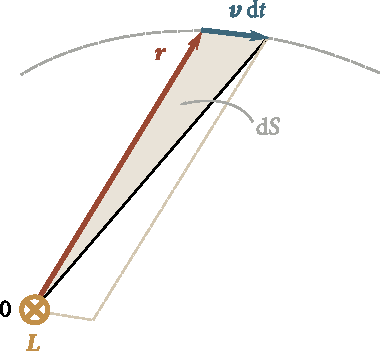
\includegraphics[scale=0.95]{figures/ch_03/fig_3_26.pdf}
			\caption[]{}
			\label{fig:3_26}
		\end{center}
	\end{minipage}
	\hspace{-0.05cm}
	\begin{minipage}[t]{0.5\linewidth}
		\begin{center}
			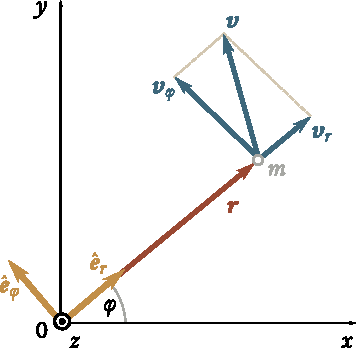
\includegraphics[scale=0.95]{figures/ch_03/fig_3_27.pdf}
			\caption[]{}
			\label{fig:3_27}
		\end{center}
	\end{minipage}
\end{figure}

\noindent
Từ đây ta kết luận rằng
\begin{equation}\label{eq:3_124}
L_z = mr^2\dot{\varphi}
\end{equation}

\noindent
trong đó $L_z$ là hình chiếu của momen xung lượng bằng module của biểu thức \eqref{eq:3_124}.

Bây giờ ta trở lại năng lượng của hạt. Các lực xuyên tâm là các lực bảo toàn ~\ref{sec:3_4}). Theo \eqref{eq:3_30}, công của lực bảo toàn bằng độ giảm thế năng $E_{\text{p}}$. Do đó đối với lực ~\eqref{eq:3_120} có hệ thức $\deriv{A}=-\deriv{E_{\text{p}}}$ nghĩa là
\begin{equation*}
\deriv{E_{\text{p}}} = -\deriv{A} = f(r)\vecuni{r}\,\deriv{\vec{r}} = -f(r)\,\deriv{r}.
\end{equation*}

\noindent
Lấy tích phân hệ thức này ta có
\begin{equation}\label{eq:3_125}
E_{\text{p}} = -\int f(r)\,\deriv{r}.
\end{equation}

\noindent
Từ \eqn{3_125} suy ra rằng thế năng của hạt nằm trong trường lực xuyên tâm chỉ phụ thuộc vào khoảng cách $r$ đến tâm; $E_{\text{p}}=E_{\text{p}}(r)$.

Các lực tỷ lệ nghịch với bình phương khoảng cách từ tâm lực có ý nghĩa đặc biệt. Đối với chúng hàm $f(r)$ trong công thức \eqref{eq:3_120} có dạng
\begin{equation}\label{eq:3_126}
f(r) = \frac{\alpha}{r^2}
\end{equation}

\noindent
trong đó $\alpha$ là một đại lượng không đổi ($\alpha>0$ ứng với trường hợp lực đẩy khỏi tâm, $\alpha<0$ ứng với trường hợp lực hút vào tâm). Các lực hấp dẫn và các lực Coulomb thuộc vào số các lực như thế.

Thay hàm ~\eqref{eq:3_126} vào biểu thức \eqref{eq:3_125} cho:

\begin{equation*}
E_{\text{p}} = -\alpha \int \frac{\deriv{r}}{r^2} = \frac{\alpha}{r} + C
\end{equation*}

\noindent
trong đó $C$ là một hằng số tích phân. Người ta thường quy ước coi thế năng ở vô cùng (tức là với $r=\infty$) bằng không. Với điều kiện này $C=0$, cho nên
\begin{equation}\label{eq:3_127}
E_{\text{p}} = \frac{\alpha}{r}.
\end{equation}

\noindent
Như vậy, cơ năng toàn phần của hạt chuyển động trong trường lực xuyên tâm tỷ lệ nghịch với bình phương khoảng cách được xác định bằng biểu thức
\begin{equation}\label{eq:3_128}
E = \frac{mv^2}{2} + \frac{\alpha}{r}.
\end{equation}

\noindent
Theo \eqn{3_122} thay bình phương vận tốc  $\vec{v}$  bằng tổng các bình phương của các vận tốc $\vec{v}_r$ và $\vec{v}_{\varphi}$, nghĩa là thay biểu thức $r^2+r^2\dot{\varphi}^2$ cho $v^2$, ta được:
\begin{equation}\label{eq:3_129}
E = \frac{m\dot{r}^2}{2} + \frac{mr^2\dot{\varphi}^2}{2} + \frac{\alpha}{r}.
\end{equation}

Trong trường xuyên tâm năng lượng và momen xung lượng của hạt được bảo toàn. Do đó các vế trái của các công thức ~\eqref{eq:3_124} và \eqref{eq:3_129} là các hằng số. Như vậy ta đi tới hệ hai phương trình vi phân; 
\begin{equation}\label{eq:3_130}
\begin{cases}
\quad\quad\quad\quad\,\,\,\,\, mr^2\dot{\varphi}^2 \!\!\!\!&= L_z = \text{constant}\\
m\dot{r}^2 + mr^2\dot{\varphi}^2 + \dfrac{2\alpha}{r} \!\!\!\!&= 2E = \text{constant}.
\end{cases}
\end{equation}

\noindent
Lấy tích phân các phương trình này, có thể tìm được $r$ và $\varphi$ như những hàm của $t$, nghĩa là tìm được quỹ đạo và đặc tính chuyển động của hạt. Ta chú ý là các đạo hàm bậc nhất theo thời gian của $r$ và $\varphi$ đều tham gia vào các \eqn{3_130}. Do đó giải chúng dễ hơn nhiều so với giải các phương trình suy từ các định luật Newton có chứa các đạo hàm bậc hai của các tọa độ.

\begin{figure}[!htb]
	%	\hspace{-0.5cm}
	\begin{minipage}[t]{0.5\linewidth}
		\begin{center}
			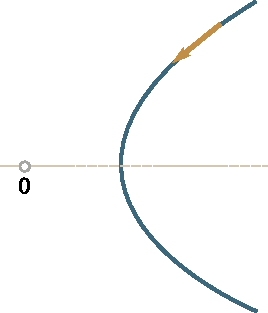
\includegraphics[scale=1]{figures/ch_03/fig_3_28.pdf}
			\caption[]{}
			\label{fig:3_28}
		\end{center}
	\end{minipage}
	\hspace{-0.2cm}
	\begin{minipage}[t]{0.5\linewidth}
		\begin{center}
			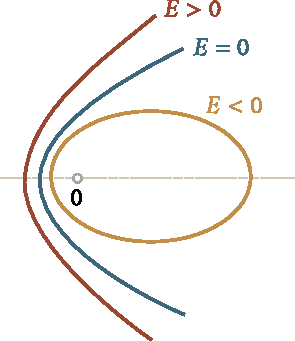
\includegraphics[scale=1]{figures/ch_03/fig_3_29.pdf}
			\caption[]{}
			\label{fig:3_29}
		\end{center}
	\end{minipage}
\end{figure}

Cách giải hệ~\eqref{eq:3_130} đi ra ngoài phạm vi cuốn sách này. Ta hạn chế ở chỗ là đưa vào kết quả cuối cùng. Quỹ đạo của hạt là một tiết diện conic, nghĩa là một elip hoặc một parabol hoặc một hypecbol. Đường nào trong các đường cong này được quan sát trong trường cụ thể đã cho, tùy thuộc vào dấu của hằng số $\alpha$ và độ lớn của năng lượng toàn phần của hạt.

Trong trường hợp lực đẩy (nghĩa là với $\alpha>0$), chỉ có đường hypecbol mới có thể là quỹ đạo của hạt (\fig{3_28}). Nếu $L_z=0$, hypecbol suy biến thành đường thằng mà đường kéo dài của nó đi qua tâm lực. Ta chú ý rằng khi $\alpha>0$ năng lượng toàn phần~\eqref{eq:3_128} không thể là âm.

Trong trường hợp lực hút (nghĩa là với $alpha<0$), năng lượng toàn phần có thể là dương cũng như âm; đặc biệt nó có thể bằng không. Khi $E>0$ quỹ đạo là một hypecbol (\fig{3_29}). Khi $E=0$ quỹ đạo là một parabol. Trường hợp này được thực hiện, nếu hạt bắt đầu chuyển động từ trạng thái nghỉ ra vô cùng (xem \eqref{eq:3_128}). Cuối cùng, khi $E<0$ quỹ đạo sẽ là một ellip. Với các giá trị của năng lượng và momen xung lượng thỏa mãn điều kiện $E=- m\alpha^2/(2L^2)$ thì elip suy biến thành đường tròn.

Chuyển động theo đường elip là chuyển động hữu hạn, chuyển động theo các đường parabol và hypecbol là chuyể động vô hạn (xem~\ref{sec:3_9}).

\section{Bài toán hai vật}\label{sec:3_19}

Bài toán về chuyển động của hai hạt tương tác lẫn nhau được gọi là \textbf{bài toán hai vật}. Hệ tạo bởi các hạt được giả thiếu là hệ kín. Trong mục~\ref{sec:3_10} đã làm rõ rằng khối tâm của hệ kín sẽ hoặc đừng nghỉ hoặc chuyển động thẳng và đều. Ta hãy giải bài toán trong hệ khối tâm (hệ k-t) bằng cách đặt gốc tọa độ tại điểm $C$. Trong trường hợp này $r_{\text{C}}=(m_1\vec{r}_1+m_2\vec{r}_2)/(m_1+m_2)=0$, nghĩa là 
\begin{equation}\label{eq:3_131}
m_1\vec{r}_1 = -m_2\vec{r}_2
\end{equation}

\noindent
(\fig{3_30}a). Ta đưa vào vector
\begin{equation}\label{eq:3_132}
\vec{r} = \vec{r}_2 - \vec{r}_1
\end{equation}

\noindent
xác định vị trí của hạt thứ hai đối với hạt thứ nhất (Hình~\ref{fig:3_30}b). Giải đồng thời~\eqref{eq:3_131} và~\eqref{eq:3_132}, dễ dàng tìm được 
\begin{equation}\label{eq:3_133}
\vec{r}_1 = -\frac{m_2}{m_1+m_2}\vec{r},\quad \vec{r}_2 = \frac{m_1}{m_1+m_2}\vec{r}.
\end{equation}
Tương tự~\eqn{3_59} có thể viết là $\vec{F}_{12}=-\vec{F}_{21}=f(r)\vecuni{r}$, trong đó $f(r)$ là hàm của khoảng cách giữa các hạt: dương đối với lực hút (\fig{3_30}c) và âm đối với các lực đẩy. Ta viết phương trình chuyển động của các hạt: 
\begin{equation*}
m_1\ddot{\vec{r}}_1 = f(r)\vecuni{r},\quad m_2\ddot{\vec{r}}_2 = -f(r)\vecuni{r}
\end{equation*}

\begin{figure}[!htb]
	\begin{center}
		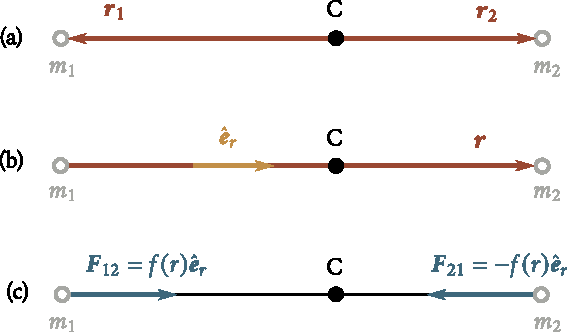
\includegraphics[scale=1]{figures/ch_03/fig_3_30.pdf}
		\caption[]{}
		\label{fig:3_30}
	\end{center}
\end{figure}

\noindent
Ta chia phương trình thứ nhất cho $m_1$, còn phương trình thứ hai cho $m_2$ và sau đó trừ phương trình thứ hai cho phương trình thứ nhất. Kết quả ta có:
\begin{equation*}
\ddot{\vec{r}}_1 - \ddot{\vec{r}}_2 = -\left(\frac{1}{m_1}+\frac{1}{m_2}\right)f(r)\vecuni{r}.
\end{equation*}

\noindent
Theo~\eqn{3_132},vế trái là $\ddot{\vec{r}}$. Như vậy,
\begin{equation}\label{eq:3_134}
\ddot{\vec{r}} = -\left(\frac{1}{m_1}+\frac{1}{m_2}\right)f(r)\vecuni{r}.
\end{equation}

\noindent
Có thể coi một cách hình thức phương trình~\eqref{eq:3_134} như phương trình chuyển động của một hạt tưởng tượng trong trường lực xuyên tâm. Vị trí của hạt đối với tâm của các lực được xác định bằng bán kính vector $\vec{r}$. Theo~\eqref{eq:3_134} cần gán cho hạt tưởng tượng một khối lượng $\mu$ được xác định bằng điều kiện 
\begin{equation}\label{eq:3_135}
\frac{1}{\mu} = \frac{1}{m_1} + \frac{1}{m_2}
\end{equation}

\noindent
Từ đây,
\begin{equation}\label{eq:3_136}
\mu = \frac{m_1m_2}{m_1+m_2}.
\end{equation}

\noindent
Đại lượng~\eqref{eq:3_136} được gọi là \textbf{khối lượng rút gọn} của các hạt.

Như vậy, bài toán hai vật được đưa về bài toán về chuyển động của một hạt trong trường lực xuyên tâm. Từ~\eqn{3_134} nếu tìm được $\vec{r}$ như hàm của $t$ thì có thể xác định $\vec{r}_1(t)$ và $\vec{r}_2(t)$ theo các công thức~\eqref{eq:3_133}. Các vector $\vec{r}_1$ và $\vec{r}_2$ được vẽ từ khối tâm $C$ của hệ. Do đó để có thể sử dụng cho công thức~\eqref{eq:3_133} cũng cần phải vẽ bán kính vector $\vec{r}$ của hạt tưởng tượng từ điểm $C$ (đối với các hạt thực thì vector~\eqref{eq:3_132} được vẽ từ hạt thứ nhất tới hạt thứ hai).

Từ các công thức~\eqref{eq:3_133} và \fig{3_30} rõ rằng là cả hai hạt chuyển động với khối tâm theo các quỹ đạo\footnote{Trong trường hợp khi lực tương tác tỷ lệ nghịch với bình phương khoảng cách giữa các hạt, thì các quỹ đạo này là các elip hoặc hypecbol (xem~\ref{sec:3_13}.)} đồng dạng hình học với nhau, hơn nữa đường thẳng nối các hạt luôn luôn đi qua khối tâm.
